\documentclass[9pt, landscape, a4paper]{article}

\usepackage{fontspec}
\renewcommand{\normalsize}{\fontsize{9}{11}\selectfont}
\usepackage[english]{babel}
\babelfont{rm}{Noto Sans}
\babelfont{sf}{Noto Sans}

\usepackage{amsmath}
\usepackage{amssymb}
\usepackage{hyperref}
\usepackage{url}
\usepackage{graphicx}
\usepackage{geometry}
\usepackage{enumitem}
\usepackage{parskip}
\usepackage{chemfig}
\usepackage{pdfpages}
\usepackage{eso-pic}
\usepackage{xcolor}
\usepackage{tikz}
\usepackage{fancybox}
\usepackage{makecell}
\usepackage{pgfplots}
\usepackage{ulem}
\usepackage{wrapfig}
\usepackage{subcaption}
\usepackage{esvect}
\usepackage{siunitx}
\usepackage{mathtools}
\usepackage{varwidth}
\usepackage{multicol}
\usepackage{titlesec}
\usepackage{bm}
\usepackage{forest}
\usepackage{upgreek}
\usepackage{tabularx}
\usepackage{booktabs}
\usepackage{colortbl}
\usepackage[column=O]{cellspace}
\usepackage{tcolorbox}

\usetikzlibrary{arrows, arrows.meta}
\usetikzlibrary{decorations.pathreplacing}
\usetikzlibrary{decorations.markings}
\usetikzlibrary{patterns}
\pgfplotsset{compat=1.18}
\definecolor{darkgreen}{rgb}{0.0, 0.6, 0.0}
\DeclareMathOperator\arctanh{arctanh}

% ============= TABLE COLORS =============
\definecolor{col1}{RGB}{80,60,160}
\definecolor{col2}{RGB}{40,140,60}
\definecolor{col3}{RGB}{50,80,180}
\definecolor{col4}{RGB}{200,100,0}
\definecolor{headerblue}{RGB}{220,230,245}
\definecolor{headertxt}{RGB}{40,60,120}
\definecolor{notebg}{RGB}{255,248,220}
\definecolor{noteborder}{RGB}{200,160,0}

% ============= GEOMETRY =============
\geometry{
    a4paper,
    landscape,
    left=0.5cm,
    right=0.5cm,
    top=1.5cm, 
    bottom=0cm,
    footskip=0cm
}

\setlist{nosep, leftmargin=*}

\AtBeginDocument{
  \setlength{\abovedisplayskip}{3pt}
  \setlength{\belowdisplayskip}{3pt}
  \setlength{\abovedisplayshortskip}{0pt}
  \setlength{\belowdisplayshortskip}{0pt}
}

% ============= HEADER & TITLES =============
\usepackage{fancyhdr}
\pagestyle{fancy}
\fancyhf{}
\rhead{\small \vspace*{.1cm}Sustainable Energy Systems Cheatsheet}
\lhead{\small \vspace*{.1cm}Matteo Frongillo}
\cfoot{\small \vspace*{.4cm}\thepage}
\newcommand{\TotalPages}{10}
\cfoot{\small \thepage/\TotalPages}
\renewcommand{\headrulewidth}{0pt}
\setlength{\headsep}{4pt}

\titlespacing*{\part}{0pt}{2pt}{1pt}
\titlespacing*{\section}{0pt}{2pt}{1pt}
\titlespacing*{\subsection}{0pt}{2pt}{1pt}
\titlespacing*{\subsubsection}{0pt}{1pt}{1pt}

\titleformat{\part}{\large\bfseries\color{black}}{}{0em}{}
\titleformat{\section}{\bfseries\color{red!80}}{}{0em}{}
\titleformat{\subsection}{\small\bfseries\color[HTML]{007AFF}}{}{0em}{}
\titleformat{\subsubsection}{\small\bfseries\color[HTML]{007355}}{}{0em}{}

% ============= META DATA =============
\newcommand{\pdftitle}[1]{\hypersetup{
  colorlinks=true,
  linkcolor=black,
  urlcolor=blue,
  pdftitle={#1},
  pdfauthor={Matteo Frongillo}
}}

% ============= RENEW COMMANDS =============

\makeatletter
\renewcommand{\author}[1]{%
  \def\@author{%
    #1\\
    \parbox{\textwidth}{%
      \centering
      \small Last update: \today
    }
  }%
}
\makeatother

\let\emptyset\varnothing

\makeatletter
\pgfmathdeclarefunction{arctan}{1}{%
    \begingroup
    \pgfmathparse{rad(atan(#1))}%
    \endgroup
}
\makeatother

\renewcommand{\tau}{\uptau}
\renewcommand{\nu}{\upnu}
\let\mathto\to
\renewcommand{\to}{\ensuremath{\mathto}\ }
% ============= NEW COMMANDS =============

\newtcolorbox{exercisebox}[1][Exercise]{
  colback=gray!5,
  colframe=gray!75!black,
  coltitle=white,
  colbacktitle=gray!75!black,
  title={\footnotesize\textbf{#1}},
  fontupper=\footnotesize,
  boxrule=0.6pt,
  arc=2pt,
  left=4pt,
  right=4pt,
  top=3pt,
  bottom=3pt
}

\newcommand{\figbox}[1]{ 
  \begin{center}
    \fbox{\begin{varwidth}{\textwidth} #1 \end{varwidth}} 
  \end{center}       
}

\newcommand{\wrapfill}{
    \par
    \ifnum \value{WF@wrappedlines} > 0
        \addtocounter{WF@wrappedlines}{-1}%
        \null\vspace{
            \arabic{WF@wrappedlines}
            \baselineskip
        }
        \WFclear
    \fi
    \phantom{}
}

\ExplSyntaxOn
\DeclareDocumentCommand{\integral}{d[] d[] d[] d[]}
{
    \IfNoValueTF{#3}{
        \IfNoValueTF{#4}{
            \displaystyle \int #1\,d#2
        }{
            \text{Error: either 2 or 4 arguments must be provided}
        }
    }{
        \IfNoValueTF{#4}{
            \text{Error: either 2 or 4 arguments must be provided}
        }{
            \displaystyle
            \int\limits
                \IfNoValueF{#1}{\c_math_subscript_token{#1}}
                ^{\IfNoValueTF{#2}{}{#2}}
                #3\, d#4
        }
    }
}
\ExplSyntaxOff

\newcommand*\circled[1]{\tikz[baseline=(char.base)]{
            \node[shape=circle,draw,inner sep=1pt] (char) {\small #1};}}

\makeatletter
\newcommand*{\rom}[1]{\expandafter\@slowromancap\romannumeral #1@}
\makeatother

\makeatletter
\newcommand{\shorteq}{\mathrel{\mkern0.2mu\mathpalette\shorteq@\relax\mkern0.2mu}}
\newcommand{\shorteq@}[2]{\scalebox{0.5}[1]{$\m@th#1=$}}

\newcommand{\longeq}[1]{\mathrel{\mathpalette\longeq@{#1}}}
\newcommand{\longeq@}[2]{%
  \begingroup
  \sbox\z@{$\m@th#1=$}%
  \ifdim#2<\wd\z@
    \resizebox{#2}{\height}{\box\z@}%
  \else
    \ifdim#2<3\wd\z@
      \hbox to #2{$\m@th#1=\hss=\hss=\hss=$}%
    \else
      \hbox to #2{$\m@th#1=\cleaders\hbox to 0.2\wd\z@{\hss$#1=$\hss}\hfil=$}%
    \fi
  \fi
  \endgroup
}
\makeatother

\newcommand{\const}{%
  \ \mathrel{\ooalign{%
    \hfil$c$\hfil\cr
    \hfil\kern0.10em\raisebox{-0.4ex}{\rule{0.08pt}{1.7ex}}\hfil\cr
  }}%
}

\makeatletter
\define@key{Gin}{lw}[1]{\setkeys{Gin}{width=#1\linewidth}}
\newcommand{\lw}{lw}
\makeatother

\newcommand{\difference}{\,\backslash\,}
\newcommand{\rem}{\underline{Remark}: }
\newcommand{\nots}{\underline{Notation}: }
\newcommand{\note}{\underline{Note}: }
\newcommand{\prf}{\underline{Proof}: }
\newcommand{\exs}{\underline{Example}: }
\newcommand{\defs}{\underline{Definition}: }
\newcommand{\wrn}{\underline{Warning}: }
\newcommand{\sht}{\ |\ }
\newcommand{\pph}[1]{\paragraph{#1} \phantom{}\\}
\newcommand{\dm}{\displaystyle}
\newcommand{\rad}{^{\mathrm{c}}}
\newcommand{\dsum}[2]{\displaystyle \sum_{#1}^{#2}}
\newcommand{\dx}[2]{\dfrac{{\mathrm{d}}^{#1}{#2}}{\mathrm{d}x^{#1}}}
\newcommand{\der}[2]{\dfrac{{\mathrm{d}}{#1}}{\mathrm{d}{#2}}}
\newcommand{\cel}{\ensuremath{^\circ}C}
\newcommand{\todo}{{\color{red}TODO}}
\newcommand{\hr}{\vspace{0.1cm}\par\vspace{-.5\ht\strutbox}\noindent\rule{\linewidth}{.5pt}\par\vspace{0.1cm}}

\DeclareMathOperator{\rot}{rot}

% ============= DOCUMENT CONTENT =============

\begin{document}
\pdftitle{Sustainable Energy Systems}

\clearpage
\includepdf[pages=1,pagecommand={\thispagestyle{empty}}]{media/SES-Cheatsheet.pdf}
\clearpage
\thispagestyle{empty}
\AddToShipoutPictureBG*{%
  \AtPageLowerLeft{%
    \includegraphics[page=2,width=\paperwidth,height=\paperheight]{media/SES-Cheatsheet.pdf}%
  }%
}

\vspace*{-.8cm}
\setlength{\columnsep}{0.5cm}
\begin{multicols*}{3}
\raggedcolumns
\null\vfill\columnbreak
\null\vfill\columnbreak

\vspace*{8.25cm}
\noindent\rule{\columnwidth}{0.5pt}

\part{SW 6: PtX and Syn Fuels}
\section{Power to X (PtX)}
PtX: conversion of excess electricity into other useful products.
\subsection{Main PtX types}
\begin{itemize}
  \item \textbf{Power-to-Gas}: H$_2$, CH$_4$
  \item \textbf{Power-to-Heat}: heat from electricity
  \item \textbf{Power-to-Fuel}: liquid fuels (eg. methanol)
  \item \textbf{Power-to-Chemicals}: feedstock (eg. ammonia, syngas)
\end{itemize}

\subsection{Purpose of PtX}
\begin{itemize}
  \item Convert excess renewable electricity for long-term storage
  \item Stabilize the grid and reduce seasonal energy gaps
  \item Increase energy system resilience
\end{itemize}

\subsubsection{Advantages}
Long-term storage, high energy density, scalable to MW range

\subsection{PtX concept}
\subsubsection{Electrolysis}
\begin{center}
  \chemfig{H_2O + electricity \rightarrow\ H_2}
\end{center}

\subsubsection{Hydrogen path}
Stored H$_2$ feeds fuel cells to produce electricity and heat

\subsubsection{Methane path + use}
\begin{center}
  \chemfig{H_2 + CO_2 \rightarrow\ CH_4}
\end{center}
Stored CH$_4$ supplies gas demand and supports electricity / heat production

\section{Electrolysis (hydrogen production)}
\subsection{Chemical reaction and energy relation}
\begin{center}
  \chemfig{{H_2O} + {E_{el}} + {E_{th}} \rightarrow\ H_2 + \frac{1}{2}O_2}
  \[\Delta_r H = \Delta_r G + T\Delta_r S\]
\end{center}

\subsubsection{Enthalpy}
\begin{itemize}
  \item $\Delta_r H$ (25\cel, atm) = 285.83 kJ/mol$_{H_2O}$: total energy demand
  \item Endothermic: $\Delta_r H > 0$
\end{itemize}

\subsubsection{Gibbs free energy}
\begin{itemize}
  \item $\Delta_r G$ (25\cel, atm) = 237.13 kJ/mol$_{H_2O}$: min. electrical energy
  \item Non-spontaneous: $\Delta_r G > 0$
\end{itemize}

\subsubsection{Reversible cell voltage}
\[U_\text{rev} = -\frac{\Delta_r G}{zF} = -1.23 V\]

\subsection{Hydrogen properties}
\begin{itemize}
  \item Highly flammable, much lighter than air
  \item Highest gravimetric energy density: 33.3 kWh/kg
  \item Low volumetric energy density: 3 kWh/m$^3$
\end{itemize}

\subsection{Water electrolysis}
Water is split using electricity. Hydrogen is produced at the cathode,
Oxygen is produced at the anode.

\subsubsection{Ion formation}
\begin{center}
  \chemfig{4H_2O \rightarrow\ 4H^{+} + 4OH^{-}}
\end{center}

\subsubsection{Cathode = reduction}
\begin{center}
  \chemfig{4H^{+} + 4e^{-} \rightarrow\ 4H}$\quad ; \quad$\chemfig{4H \rightarrow\ 2H_2}
\end{center}

\subsubsection{Anode = oxidation}
\begin{center}
  \chemfig{4OH^{-} \rightarrow\ 4OH + 4e^{-}}$\quad ; \quad$\chemfig{4OH \rightarrow\ 2H_2O + O_2}
\end{center}

\begin{exercisebox}[Exercise: Waste heat reuse of PEM electrolysis]
  \begin{minipage}[t]{0.48\linewidth}
    Input:
    \begin{itemize}
      \item Electricity: 204.03 MJ/kg H$_2$
      \item Water: 9.04 kg
    \end{itemize}
  \end{minipage}
  \hfill
  \begin{minipage}[t]{0.48\linewidth}
    Output:
    \begin{itemize}
      \item Hydrogen: 1 kg
      \item Oxygen: 7.94 kg
    \end{itemize}
  \end{minipage}
  \vspace{.2cm}
  \begin{enumerate}[label=\alph*.]
    \item Draw a schematic of the situation
    \item What is the cell efficiency? (LHV$_{\mathrm{H}_2}$ = 120 MJ/kg)
    \item Assuming 80\% of the waste heat can be used for another purpose. What is the exergetic efficiency of the
        electrolysis? Assuming a reaction temperature of 80\cel, ambient temperature of 25 \cel
  \end{enumerate}
  \hr
  \begin{enumerate}[label=\alph*.]
    \item 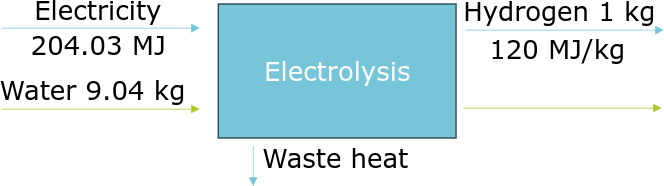
\includegraphics[\lw=.5]{media/electrolysis-exercise.png}
    \item $\eta_\text{cell} = \frac{120\text{ MJ}}{204.03\text{ MJ}} = 0.588 = 58.8\%$
    \item $Q_\text{waste} = (204.03 - 120)\text{ MJ} = 84.03\text{ MJ}$\\
      $Q_\text{waste,use} = 84.03\text{ MJ} \cdot 0.8 = 67.22\text{ MJ}$\\[.5ex]
      $EX_\text{waste,use} = 67.22\text{ MJ} \left(1 - \frac{T_0}{T}\right) = 67.22 \left(1 - \frac{298}{353}\right) = 10.49\text{ MJ}$\\[.5ex]
      $\eta_{\text{cell},EX} = \frac{120\text{ MJ} + 10.49\text{ MJ}}{204.03\text{ MJ}} = 0.6395 = 64\%$
  \end{enumerate}
\end{exercisebox}

\subsection{Types of electrolysis}
\subsubsection{AEL -- Alkaline Electrolysis}
\begin{itemize}
  \item Mature, industrial scale: > 100 MW$_\text{el}$
  \item Electrolyte: 20--40 wt\% KOH, not consumed
  \item Ni electrodes; diaphragm transports OH$^-$ and split gases
\end{itemize}

\subsubsection{PEM -- Proton Exchange Membrane}
\begin{itemize}
  \item Less mature, up to several MW$_\text{el}$; 5--10 times smaller than AEL
  \item Solid polymer membrane conducts H$^+$ and blocks electrons
  \item Acidic, anode-fed system; needs costly durable materials, eg. Nafion
\end{itemize}

\subsubsection{SOEC -- Solid Oxide Electrolysis Cell}
\begin{itemize}
  \item High-temperature steam electrolysis: 700 - 1000 \cel
  \item Heat replaces part of the electrical demand
  \item Solid oxide membrane conducts O$^{2-}$
\end{itemize}

\section{Methane}
\subsection{Pros and Cons}
\textbf{Pros}: good fuel and storage gas, higher volumetric energy density than H$_2$,
uses existing gas infrastructure, can form longer hydrocarbons.

\textbf{Cons}: Lower gravimetric energy density than H$_2$

\subsection{Methanation}
Conversion of H$_2$ and CO$_2$ into methane CH$_4$
\subsubsection{Chemical}
\begin{itemize}
  \item Sabatier reaction
  \item Converts \chemfig{CO_2 + H_2 \rightarrow\ CH_4}
\end{itemize}

\subsubsection{Biological}
\begin{itemize}
  \item Uses H$_2$
  \item Bacteria/enzymes act as catalyst
\end{itemize}

\subsection{Thermochemical methanation}
\begin{center}
  \chemfig{CO_2 + 4H_2 \rightarrow\ CH_4 + 2H_2O}
  \[\Delta_r H = \Delta_r G + T\Delta_r S\]
\end{center}
\begin{itemize}
  \item Exothermic: $\Delta_r H < 0$; 300--500\cel
  \item Ni-based catalyst, needs CO$_2$
  \item Waste heat improves efficiency
\end{itemize}

\section{Fuels}
\subsection{Fischer-Tropsch reaction}
Aims to produce sustainable liquid hydrocarbons \chemfig{C_nH_{2n+2}} from CO$_2$ and H$_2$
\subsubsection{Process}
\begin{itemize}
  \item Electrolysis \to H$_2$
  \item RWGS \to syngas CO + H$_2$
  \item FT synthesis \to liquid fuels
\end{itemize}
\subsubsection{Main products}
Kerosene, diesel, naphtha, lubricating oil

\subsection{Synhelion}
\begin{itemize}
  \item Concentrated solar heat drives fuel production
  \item TES stores heat for continuous operation
  \item \chemfig{CO_2 + H_2O \rightarrow\ CO + H_2}
  \item Syngas \to GTL/FT \to gasoline, diesel, kerosene
\end{itemize}

\section{Storage}
\begin{itemize}
  \item Tank: limited volume
  \item Porous caverns: existing tanks; scarcity, contamination risk
  \item Aquifer: abundant; needs exploration, low leak rate
  \item Rock salt caverns: large volumes, high gas purity
  \item Underground pipes: independent from geology, expensive
\end{itemize}

\section{X-t-P}
\subsection{Fuel cell}
\begin{itemize}
  \item Reverse electrolysis: \chemfig{H_2 + \frac{1}{2}O_2 \rightarrow\ H_2O + electricity}
  \item Continuous input: H$_2$ + air/O$_2$
  \item Output: water, electricity, heat
  \item Anode + cathode + electrolyte
  \item Porous electrodes for gas flow
  \item Cell voltage < 1 V \to stack needed
\end{itemize}

\subsubsection{Fuel cell types}
\begin{tabularx}{\columnwidth}{@{}lccXc@{}}
  \toprule
  \textbf{Type} & \textbf{Temp.} & \textbf{Carrier} & \textbf{Electrolyte} & \textbf{Eff.}\\
  \midrule
  AFC & 60--120\cel & OH$^-$ & KOH & 35--55\%\\
  PEMFC & 50--100\cel & H$^+$ & polymer membr. & 35--45\%\\
  SOFC & 800--1000\cel & O$^{2-}$ & zirconia & >50\%\\
  \bottomrule
\end{tabularx}

\subsubsection{Proton Exchange Membrane (PEM) fuel cell}
Polymer membrane conducts only H$^+$, not electrons:
\vspace*{-.2cm}
\begin{itemize}
  \item Anode: \chemfig{H_2 \rightarrow\ H^{+} + e^{-}}
  \item H$^+$ passes through membrane
  \item e$^-$ goes through external circuit \to current
  \item Cathode: \chemfig{H^{+} + e^{-} + O_2 \rightarrow\ H_2O}
\end{itemize}

\subsection{Combustion}
\begin{itemize}
  \item \textbf{Power generation}: fuel \to turbine \to generator
  \item \textbf{CHP}: produces electricity + useful heat
  \item CHP improves total efficiency by reusing waste heat
\end{itemize}
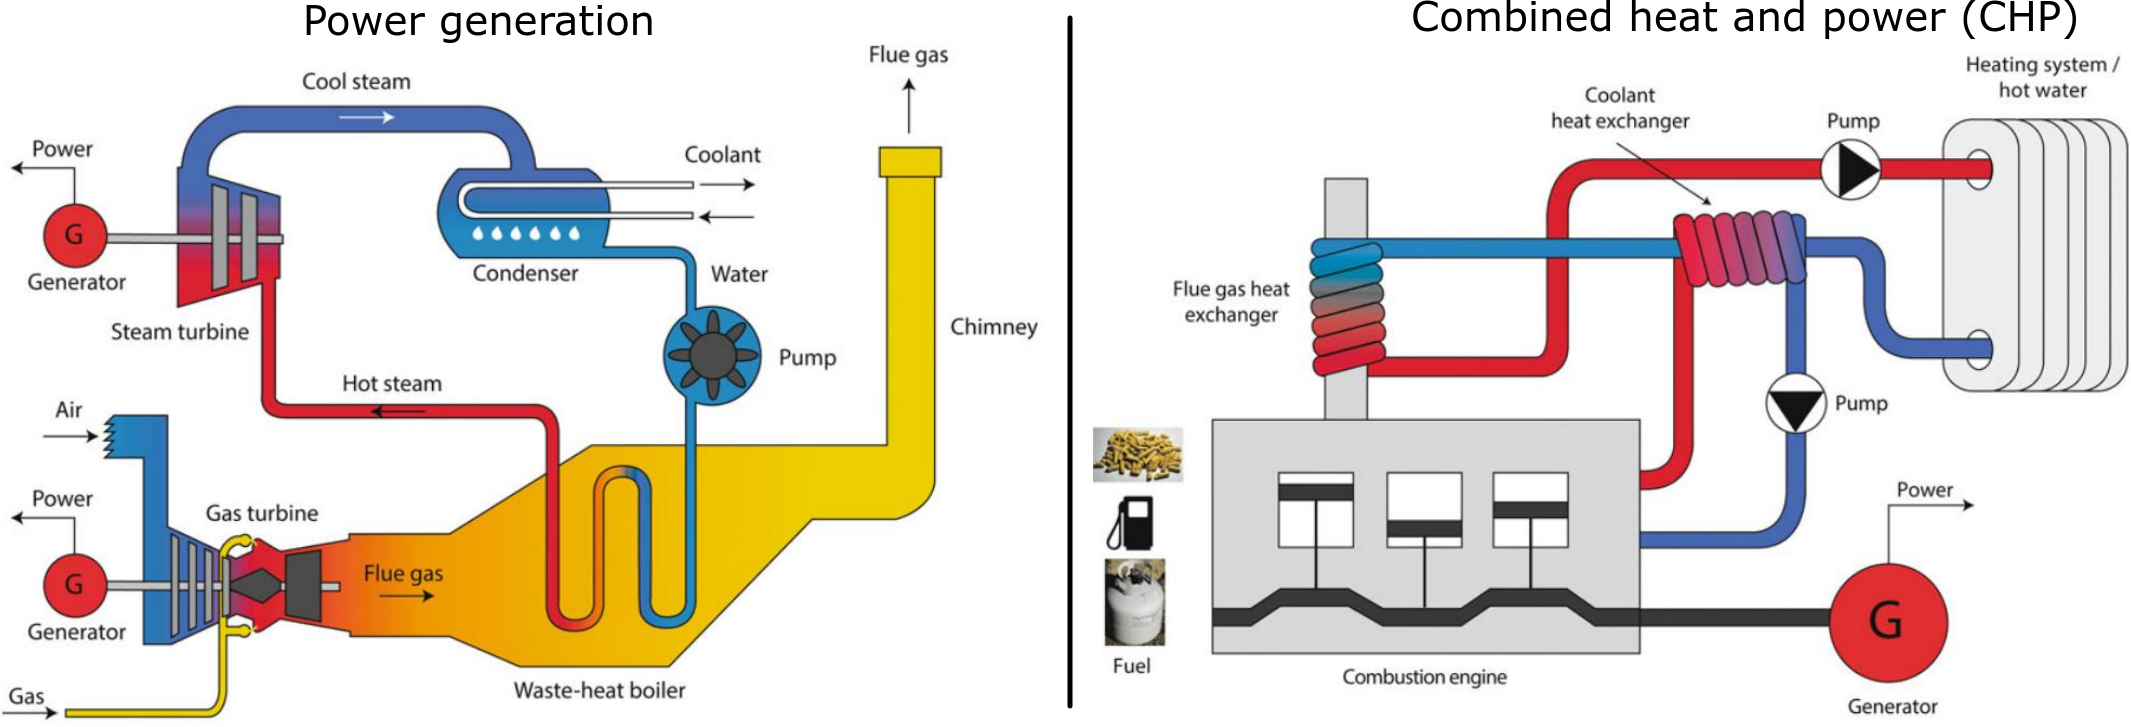
\includegraphics[\lw]{media/combustion.png}

\section{PtXtP}
PtX has low electricity-to-electricity efficiency: CH$_4$ gives only 30--38\%, while
batteries reach 80--90\%.

PtX is mainly useful for long-term storage or when gas / heat / fuels are needed, not
for short-term electricity storage.

\newcolumn
\vspace*{-.5cm}
\part{SW 8: Electrical Grids}

\section{Grid integration of renewables}
\begin{itemize}
  \item Main issues: fluctuating production, winter/day supply gaps, congestion, voltage limits
  \item More RES requires storage, smart control, grid reinforcement/expansion
  \item Switzerland: voltage issues at connection points are often more critical than transformer overloads
  \item PV curtailment: limiting peak power can lose little energy; 50\% power limit $\approx$ 10\% energy loss
\end{itemize}

\subsection{Synchronous grids}
\begin{itemize}
  \item All generators/loads operate at common frequency: Europe 50 Hz, North America 60 Hz
  \item Interconnected AC network enables power flow and trading over large areas
  \item Stability needs supply-demand balance, frequency control, voltage control, overload mitigation
  \item Large rotating machines provide inertia and slow frequency changes
  \item Alternatives: isolated grids, microgrids, DC grids, HVDC links
\end{itemize}

\subsection{DC transmission}
\begin{itemize}
  \item Connects asynchronous areas/islands; different frequencies possible
  \item Efficient for long distance $>500$ km: no reactive power losses, no skin effect
  \item Drawbacks: costly converters, harder monitoring/balancing, meshed DC grids complex
\end{itemize}

\section{Grid structure and components}
\subsection{Swiss grid levels}
Swiss transmission grid: 1 TSO, 380/220 kV, $\sim 6700$ km, substations, cross-border
links, 2.5m CHF planned investment.
\begin{center}
  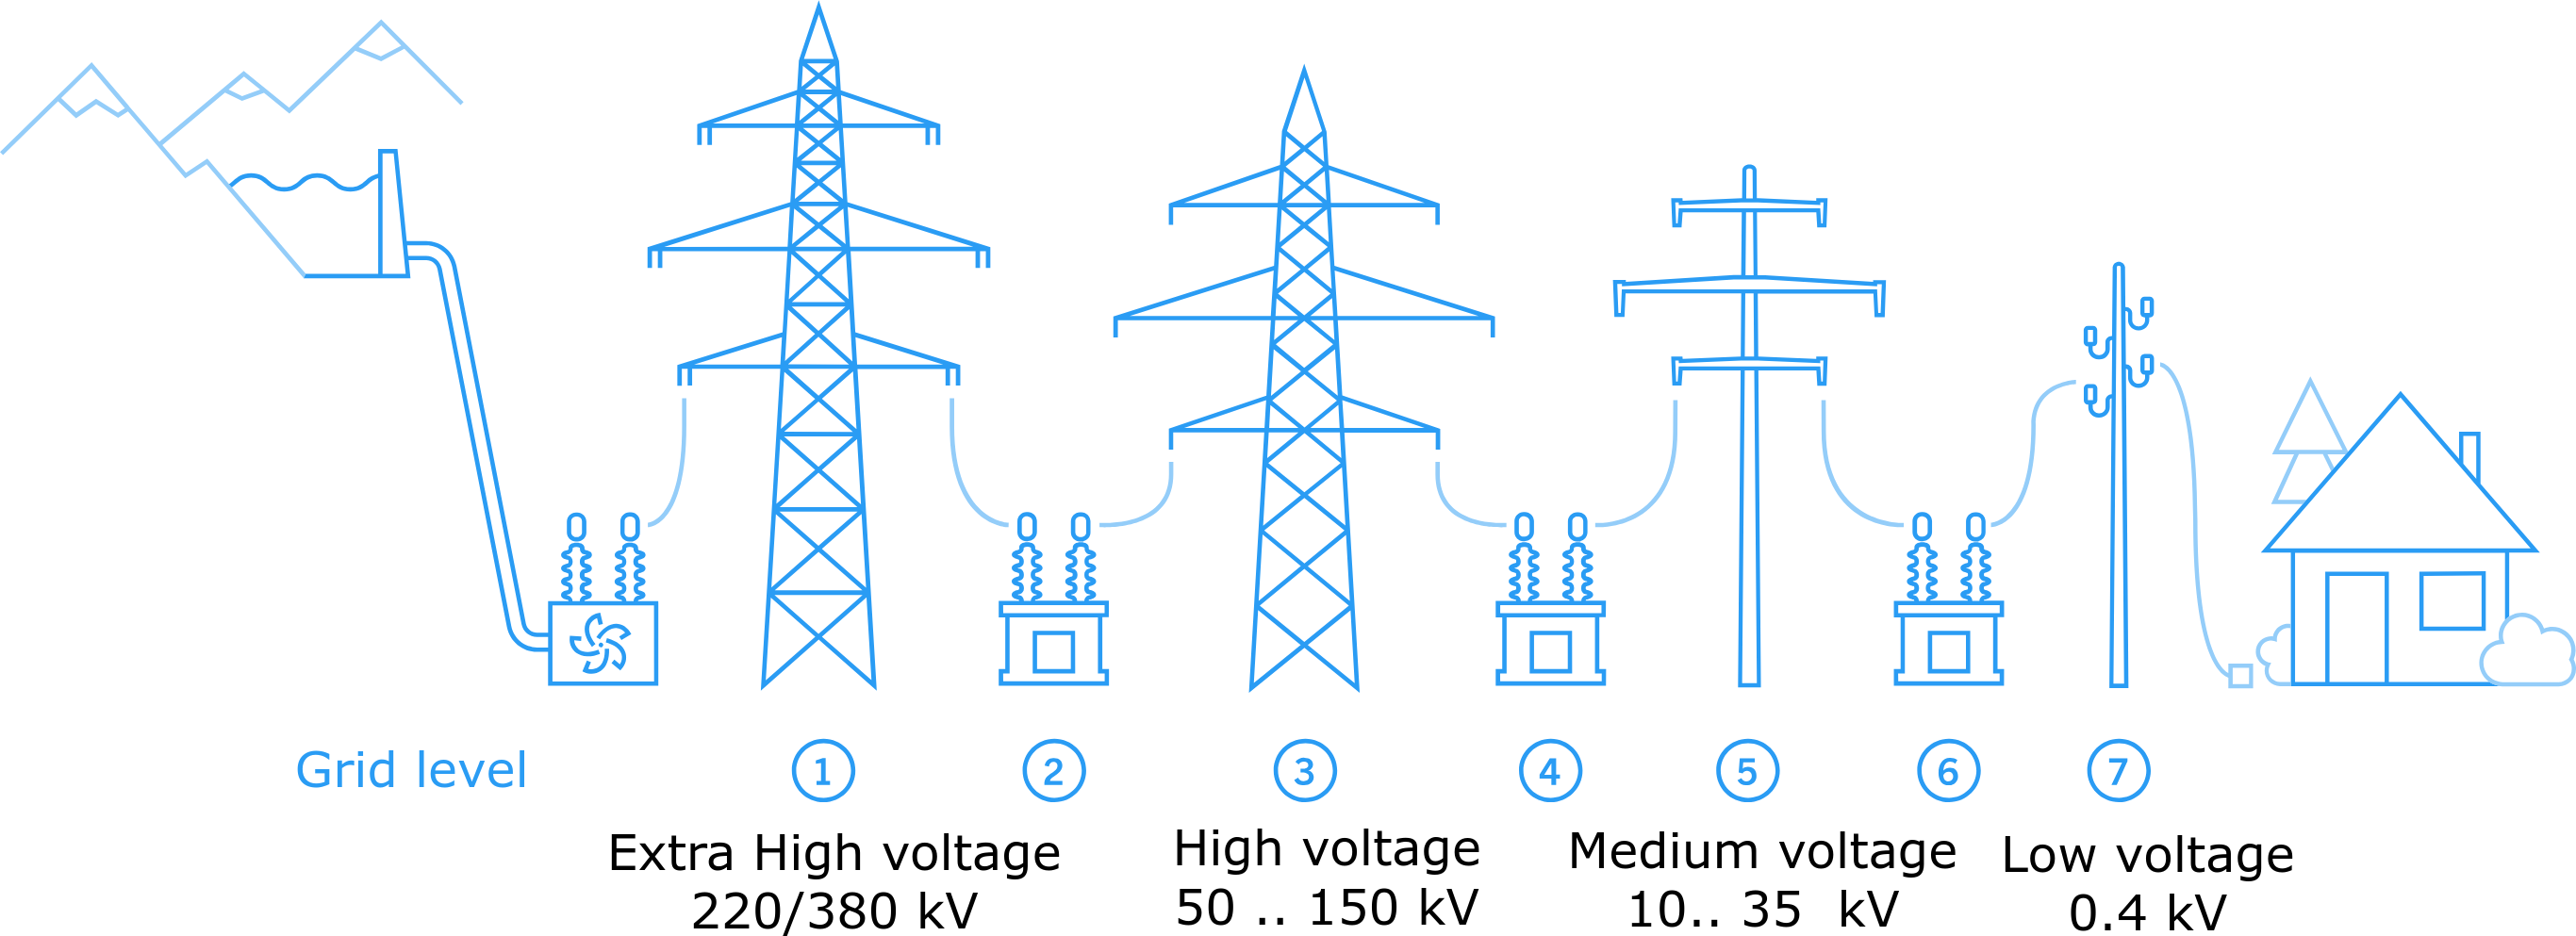
\includegraphics[\lw]{media/swiss-grid.png}
\end{center}

\subsection{Components}
\begin{itemize}
  \item Generation: hydro, nuclear, thermal, renewables
  \item Delivery: overhead lines, underground cables, substations
  \item Conversion/control: transformers, converters, tap changers, capacitor banks
  \item Storage/loads: pumped hydro, BESS, industrial and local loads
  \item Protection/monitoring: circuit breakers, fuses, SCADA, sensors, automation
\end{itemize}

\subsection{Operation requirements}
\begin{itemize}
  \item Frequency stable and in range
  \item Voltage stable and in range
  \item Operation within nominal current, voltage, thermal limits
  \item Resilience against faults/short circuits
  \item Transient stability after disturbances
  \item $n-1$ criterion: supply remains guaranteed after any single component failure
\end{itemize}

\section{Renewable Energy Sources (RES) integration measures}
\subsection{Voltage issues}
\begin{itemize}
  \item Reactive power regulation: absorb/inject $Q$ to control local voltage
  \item Active power limitation: curtail feed-in peaks
  \item Voltage regulating transformer: static or adjustable
  \item Grid reinforcement:\\lower line/transformer impedance \to lower voltage rise
\end{itemize}

\subsection{Overloading}
\begin{itemize}
  \item Increase self-consumption; synchronize local loads with local production
  \item Active power limitation: fixed feed-in limit or dynamic limit
  \item Grid reinforcement increases transport capacity and reduces impedance
\end{itemize}

\section{Power in AC lines}
\subsection{Complex power}
\[S = V I^* = P + jQ\]
where:\\
$S$: apparent/complex power [VA], $I^*$: current conjugate
\begin{itemize}
  \item Active power: $P = Re(S) = VI\cos\theta$ [W]
  \item Reactive power: $Q = Im(S) = VI\sin\theta$ [var]
  \item Power factor: $\cos\theta = P/S$
\end{itemize}

\subsection{Line impedance, Power in a transmission line, Power losses}
\[Z = R + jX\quad ;\quad S = P+jQ\frac{\left|V\right|^2}{Z}\quad ;\quad P_\text{loss} = I^2R\]
\begin{itemize}
  \item Higher voltage levels usually have higher reactance $X$
  \item Reactive power flow is inefficient in transmission grids
\end{itemize}

\section{Voltage drop/rise at a connection point}
\[\Delta U_2[\%] \approx \frac{R\,\Delta P + X\,\Delta Q}{U_n^2}\cdot 100\]
where $U_n$: rated voltage = 400 V
\vspace*{-.2cm}
\begin{itemize}
  \item $\Delta P > 0$ MW (more load) \to $\Delta U$ positive \to $U_2$ decreases
  \item $\Delta P < 0$ MW (more feed-in) \to $\Delta U$ negative \to $U_2$ increases
  \item $\Delta Q > 0$ Mvar (inductive) \to $\Delta U$ positive \to $U_2$ decreases
  \item $\Delta Q < 0$ Mvar (capacitive) \to $\Delta U$ negative \to $U_2$ increases
  \item Local feed-in/load changes voltage; high RES feed-in can cause overvoltage.
\end{itemize}

\begin{exercisebox}[Exercise: Loss in a transmission line]
  An existing 10 kV transmission line carries 2 MVA (single phase line).
  \begin{enumerate}[label=\arabic*.]
    \item How much active power can it carry at $\cos(\theta)=0.95$?
    \item What are the active power losses for $Z = 1 + j2\,\Omega$?
    \item For the same active power, what are the losses at $\cos(\theta)=0.8$?
  \end{enumerate}
  \hr
  \begin{enumerate}[label=\arabic*.]
    \item $P = S\cos\theta = 2\text{ MVA}\cdot0.95 = 1.9\text{ MW}$
    \item $I = \frac{S}{U} = \frac{2\text{ MVA}}{10\text{ kV}} = 200\text{ A}$\\
      $P_\text{loss} = I^2R = (200\text{ A})^2\cdot1\,\Omega = 40\text{ kW}$
    \item $S = \frac{P}{\cos\theta} = \frac{1.9\text{ MW}}{0.8} = 2.375\text{ MVA}$\\
      $I = \frac{S}{U} = \frac{2.375\text{ MVA}}{10\text{ kV}} = 237.5\text{ A}$\\
      $P_\text{loss} = (237.5\text{ A})^2\cdot1\,\Omega \approx 56.4\text{ kW}$
  \end{enumerate}
\end{exercisebox}

\begin{exercisebox}[Exercise: Voltage drop in a low-voltage grid]
  A 400 V LV feeder supplies a household.\\
  $R=0.15\,\Omega$, $X_L=0.1\,\Omega$, $U_n=400\text{ V}$, initial $P=5\text{ MW}$, $Q=2\text{ MVAr}$.\\
  A PV plant changes $\Delta P=-100\text{ kW}$ and voltage control sets $\Delta Q=100\text{ kVAr}$ inductive.
  \begin{enumerate}[label=\arabic*.]
    \item Calculate $\Delta U_2[\%] \approx \frac{\Delta P R + \Delta Q X_L}{U_n^2}\cdot100$
    \item Does the household voltage increase or decrease?
    \item How can voltage fluctuations be mitigated?
  \end{enumerate}
  \hr
  \begin{enumerate}[label=\arabic*.]
    \item $\Delta U_2 = \frac{(-100000)\cdot0.15 + 100000\cdot0.1}{400^2}\cdot100
      = -3.125\%$
    \item Negative voltage drop \to voltage rises by $\approx 3.13\%$:
      $\Delta U \approx 12.5\text{ V}$, so $U_2 \approx 412.5\text{ V}$
    \item Reactive power control, active power curtailment, tap changer, local load shifting/self-consumption,
      grid reinforcement
  \end{enumerate}
\end{exercisebox}

\part{SW 9+10: Mobility and Smart Grid Trends}

\section{E-mobility status quo}
\begin{itemize}
  \item Mobility uses $\approx 1/3$ of Swiss final energy; transport is still mostly fossil
  \item Electrification of transport/heating increases electricity demand; transport electricity still $<10\%$
  \item EVs: $\sim 50$--$80\%$ life-cycle CO$_2$ savings vs. combustion vehicles
  \item Switzerland: BEV/PHEV $\sim 1/3$ of new car registrations; total EV stock still low
  \item 2050: $\sim 4$--$5$ million EVs; storage potential $\sim 200$ GWh, comparable to pumped storage
  \item Policy: Climate and Innovation Act, new Electricity Act incentives for electric mobility/storage
\end{itemize}

\subsection{Role in Energy Strategy 2050}
\begin{itemize}
  \item High PV/wind share \to more fluctuating production
  \item Almost fully electrified car fleet can become flexible load and distributed storage
  \item Bidirectional charging potential depends on charger power and availability for grid services
\end{itemize}

\newcolumn
\section{Powertrains and storage}
\subsection{Powertrain comparison}
\begin{itemize}
  \item BEV: highest well-to-wheel efficiency; best suited if electricity is low-carbon
  \item FCEV/H$_2$: lower chain efficiency due to electrolysis, compression/storage, fuel cell losses
  \item ICE/H$_2$ combustion: low drivetrain efficiency; fuel handling easier than batteries
  \item BEV mid-size car life-cycle emissions much lower than ICE; lecture example $\approx 55$--$58\%$ reduction
\end{itemize}

\subsection{Battery storage}
\begin{itemize}
  \item E-mobility needs high specific energy [kWh/kg] and energy density [kWh/L]
  \item Li-ion batteries store much less energy per kg than liquid fuels, but EV drivetrain efficiency is high
  \item Typical drivetrain efficiency: EV $\sim 80\%$ vs. combustion $\sim 20\%$
  \item Li-ion battery costs fell strongly; lecture: about $-80\%/10$ yr
\end{itemize}

\subsection{Battery ageing}
\begin{itemize}
  \item Ageing types: calendar ageing and cycling ageing
  \item Drivers: temperature, C-rate, depth of discharge, energy throughput, deep discharge at high temperature
  \item V2X ageing likely low/minimal for slow grid services; warranty conditions vary by manufacturer
  \item Typical warranty: 5--8 years, 160'000--240'000 km, often $\geq 70\%$ remaining capacity
\end{itemize}

\section{Charging infrastructure}
\subsection{AC vs. DC charging}
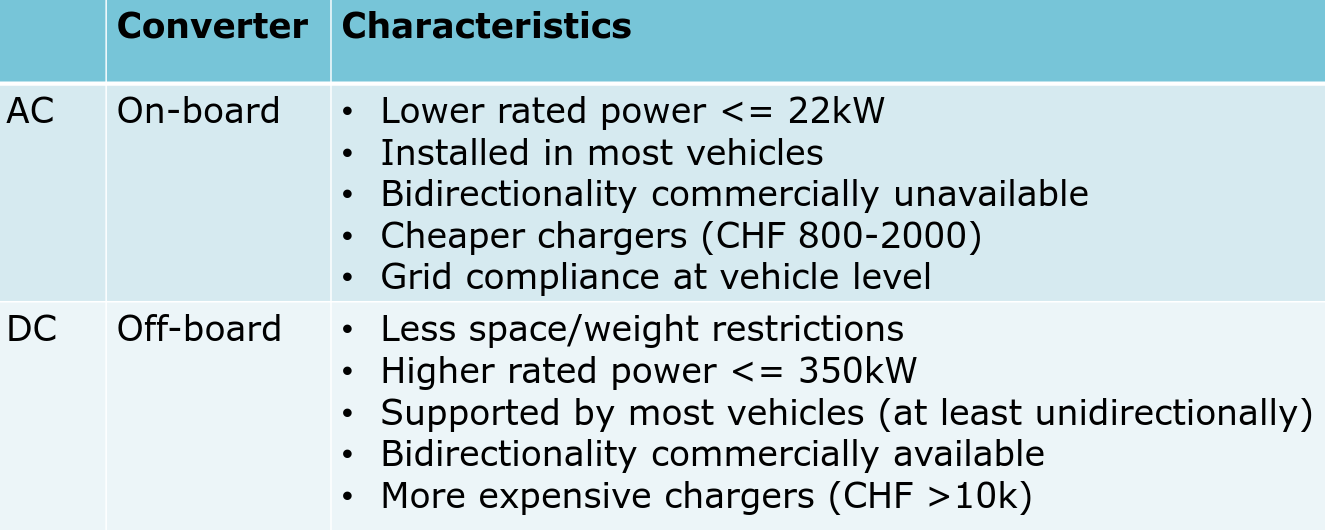
\includegraphics[\lw]{media/acdc-charging.png}
\vspace*{-.6cm}
\begin{itemize}
  \item DC bidirectional charging is commercially more available
  \item AC bidirectional still limited
  \item Requirements:\\AC/DC conversion, DC voltage regulation, galvanic isolation
  \item MCS for heavy vehicles: MW scale, up to $\sim 3.75$ MW target
\end{itemize}

\subsection{Connector types}
\subsubsection{DC connector types}
\begin{itemize}
  \item CCS: PLC communication, de facto standard in Europe/North America, bidirectional specified but limited
  \item CHAdeMO: CAN bus, bidirectional commercially available, standard in Japan, phased out in Europe
  \item Inductive charging (wireless)
\end{itemize}

\newcolumn
\begin{center}
  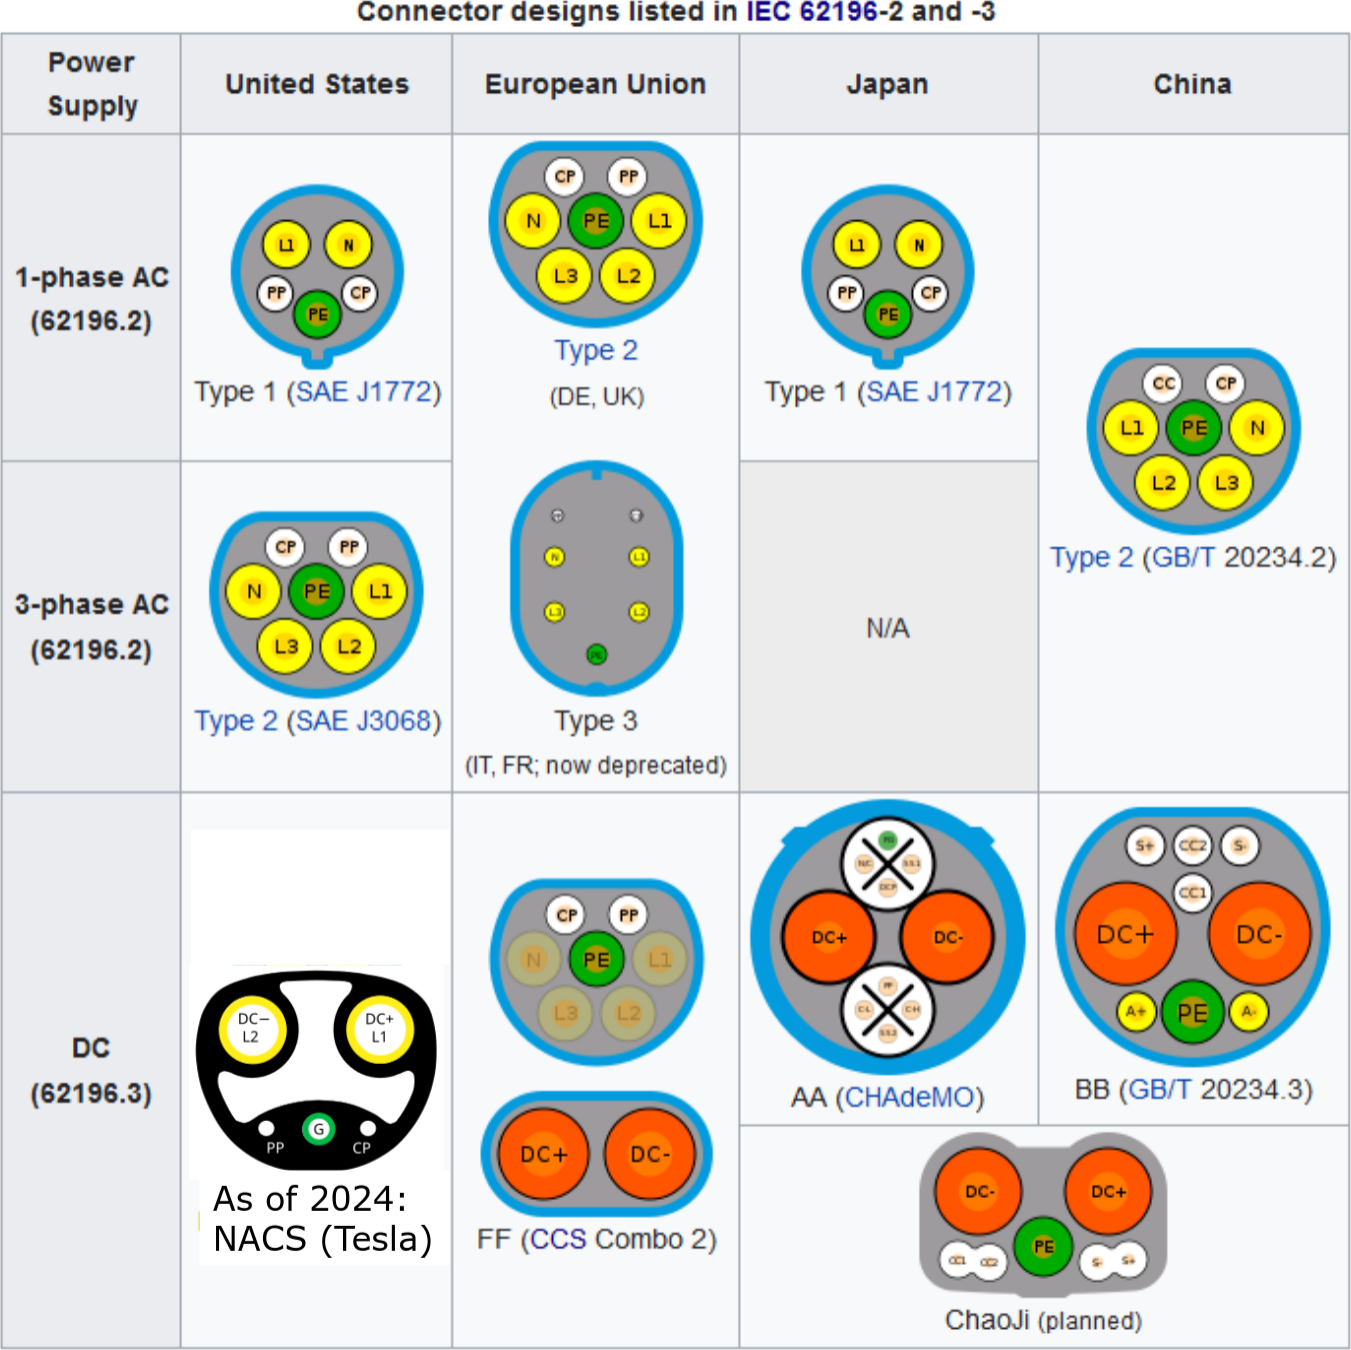
\includegraphics[\lw=.75]{media/connectors.png}
\end{center}

\subsection{IEC 61851 charging modes}
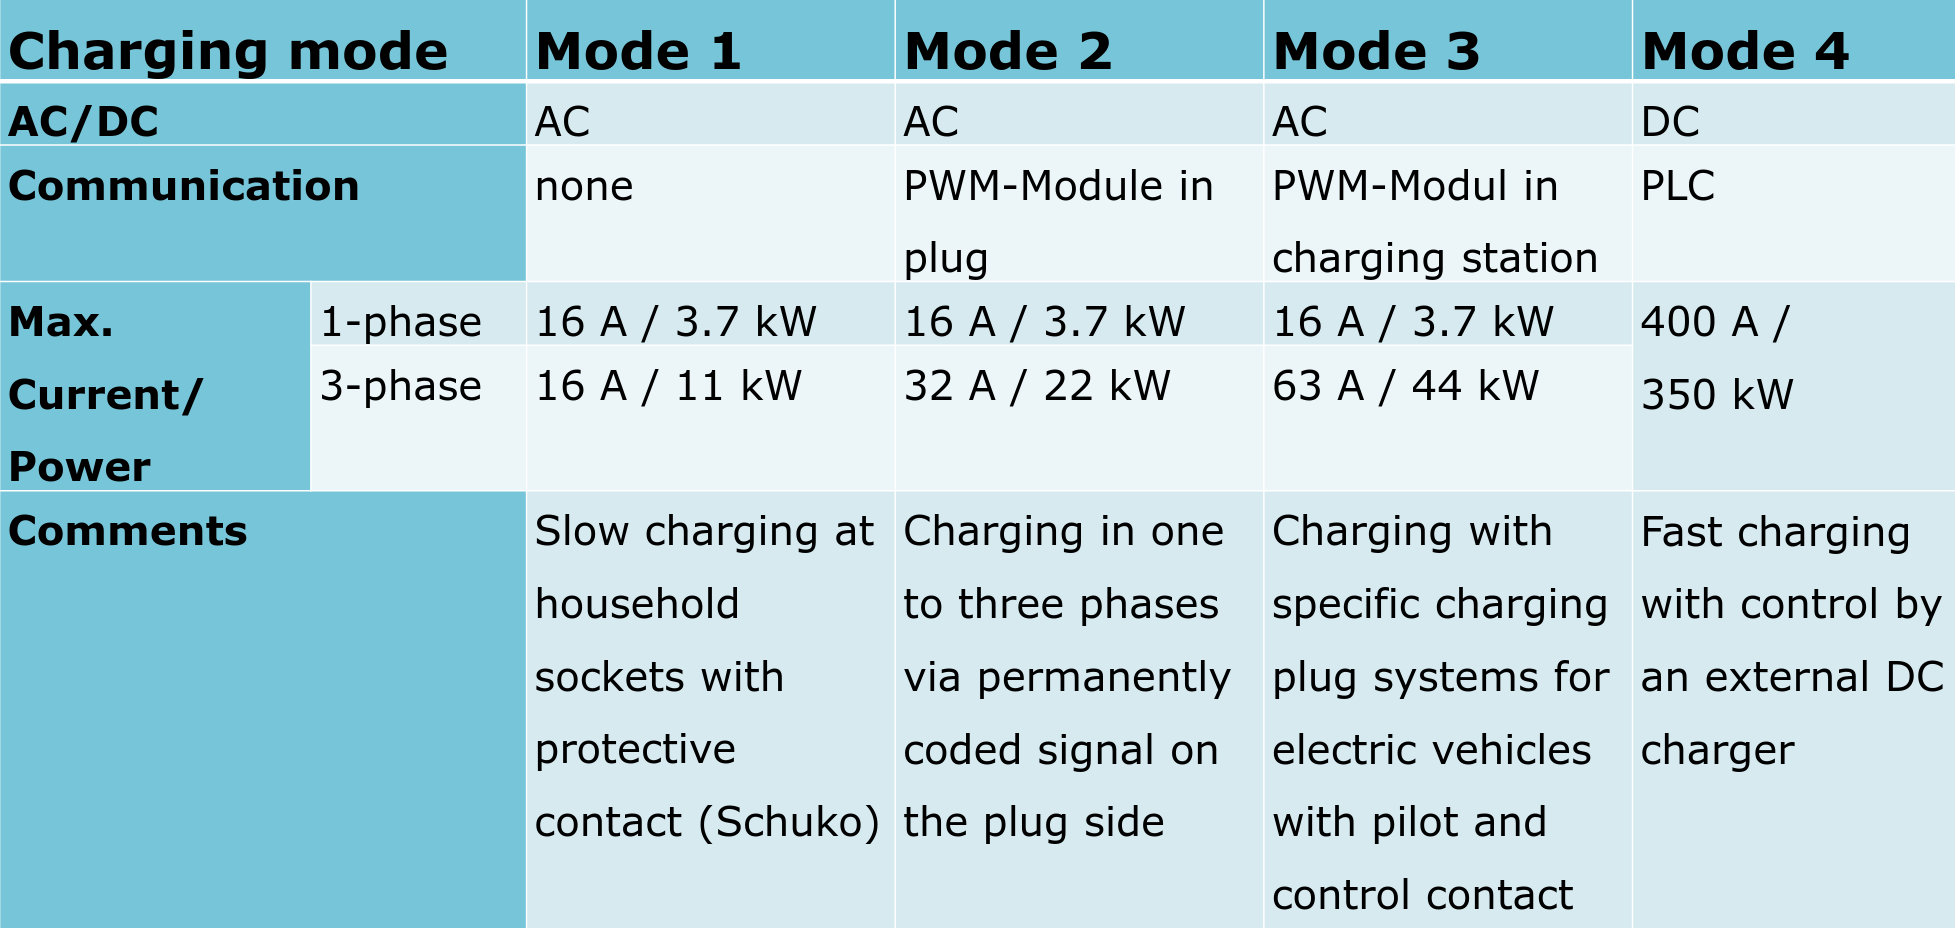
\includegraphics[\lw]{media/IEC.png}

\section{Management and interoperability}
\subsection{Charge management (local parameters)}
Charging is regulated based on several parameters:
\vspace*{-.2cm}
\begin{itemize}
  \item State of charge and temperature of the high-voltage battery
  \item Charger's power and load of the charging station (wallbox)
  \item Permissible charging power of the cable
\end{itemize}

\subsection{Load management (upstream limitations)}
\begin{itemize}
  \item Regulates the charging process within a building or area
  \item Prevents the maximum reference power at the connection point from being exceeded
  \item Other input variables are considered (eg. PV system optimisation and special tariffs)
  \item Applies to both local and higher-level load management
\end{itemize}

\subsubsection{Dynamic and static load management}
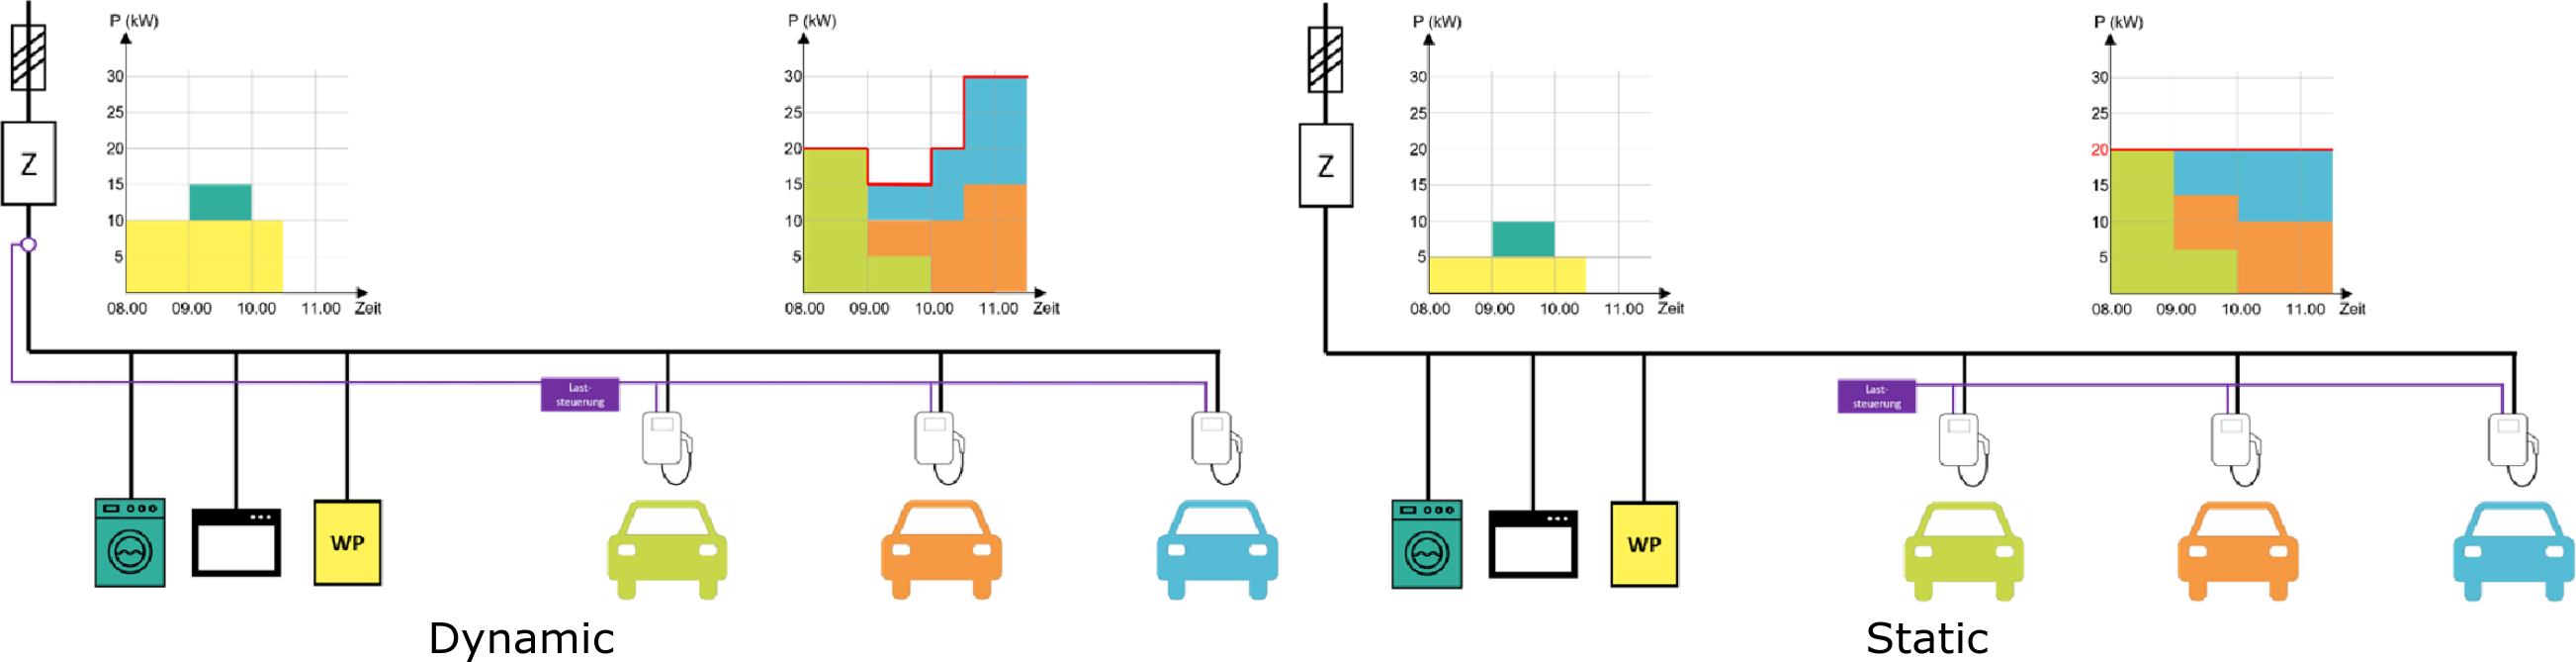
\includegraphics[\lw]{media/dyn-static.png}

\subsection{Interoperability}
\begin{itemize}
  \item Required across backend systems, charging infrastructure, vehicles, users
  \item Challenges: cybersecurity, privacy, protocols, response times, plug types, warranties, regulation
  \item No one-size-fits-all solution today; V1G/V2G compatibility depends on car, charger, backend
\end{itemize}

\section{Grid integration and Flexibility of EVs, V2X}
\subsection{Impacts of EVs on electrical power systems}
\begin{itemize}
  \item EV uptake increases energy demand and peak power consumption
  \item Superchargers create high ramp rates and local $100+$ kW power steps
  \item Risks: transformer/line overloads, congestion, higher losses, network reinforcement needs
\end{itemize}

\subsubsection{Impacts on distribution grids}
\begin{itemize}
  \item Directly affects voltage level
  \item Affects power flows in lines and transformers
  \item Reverse power flows can be challenging for sys. protection
  \item Might increase network losses
  \item Causes high ramp rates after dark (Duck curve)
\end{itemize}

\subsubsection{Challenges for distribution system operation}
\begin{enumerate}
  \item Increasing demand from EV charging
  \item Uncertainty in renewable generation
\end{enumerate}
\vspace*{-.2cm}
Mitigation: uni- and bidirectional charging; smart charging; Vehicle-to-grid (V2G) integration.

\subsection{Bidirectional charging}
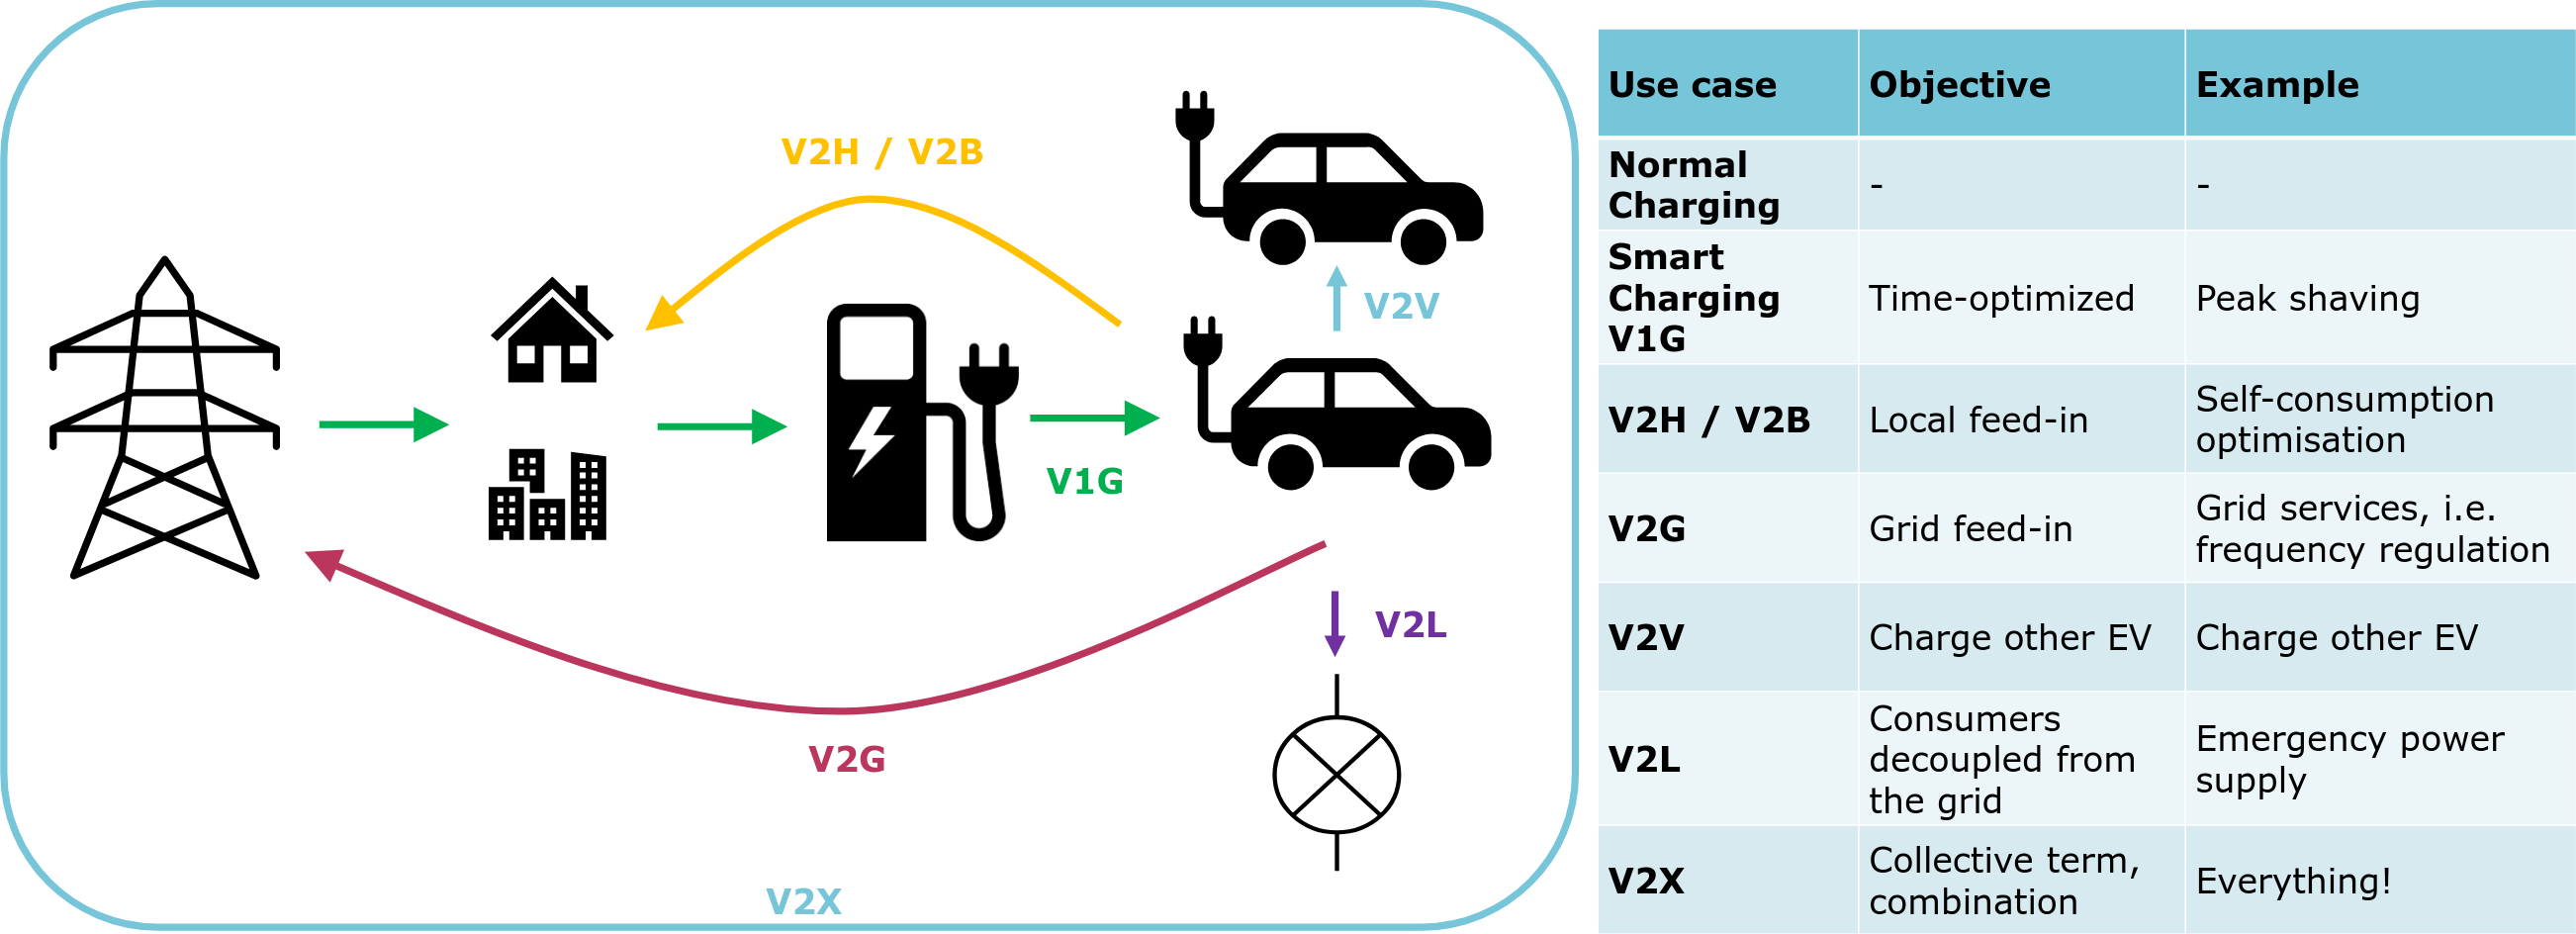
\includegraphics[\lw]{media/bidirectional.png}

\subsubsection{Use cases}
\begin{itemize}
  \item Standard charging: uncontrolled, cheap, but causes load spikes
  \item V1G / smart charging: unidirectional controlled charging; peak shaving, tariff/PV optimization
  \item V2H/V2B: vehicle supplies home/building; self-consumption, peak shaving, backup power
  \item V2G: vehicle feeds grid; frequency control, congestion management, voltage regulation
  \item V2L: loads supplied directly from vehicle; V2V: charge another vehicle; V2X: umbrella term
\end{itemize}

\subsubsection{Technology readiness}
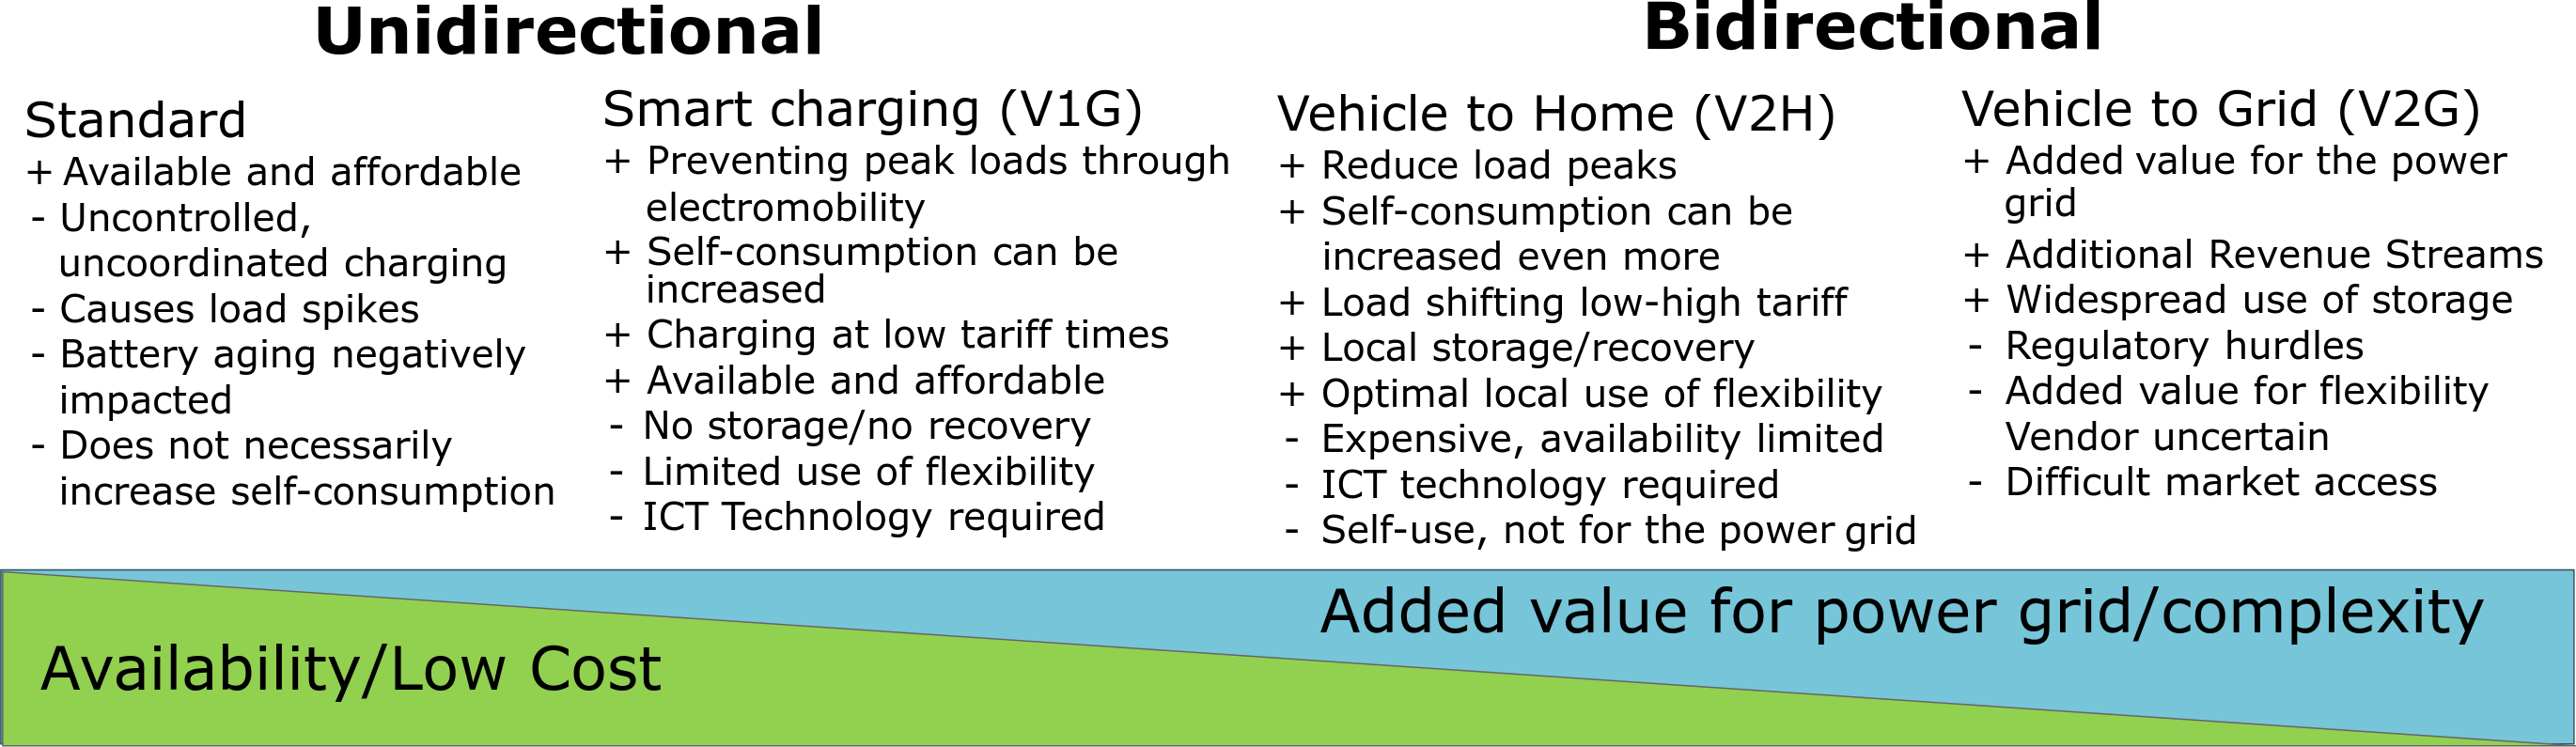
\includegraphics[\lw]{media/uni-vs-bi.png}

\subsection{Battery ageing and warranty}
\subsubsection{Ageing}
\begin{itemize}
  \item Complex, even without bidirectional charging
  \item Calendar Ageing \& Cycling Ageing
  \item Operating temperature, charge/discharge rates, depth of discharge, energy throughput \to individual use
  \item Deep discharge combined with elevated temp. \to main driver
  \item Limited experience for bidirectional charging
  \item Low discharge rates due to V2X use cases
  \item Extra V2X ageing is expected to be low; not enough to make V2X technically infeasible
\end{itemize}

\subsubsection{Warranty}
\begin{itemize}
  \item Battery warranties usually limited by both age and mileage
  \item Typical range: 5--8 years and 160'000--240'000 km
  \item End-of-warranty guarantee often requires at least 70\% remaining capacity
  \item V2X warranty treatment differs strongly by manufacturer
  \item Market is still early; warranty impact cannot yet be judged
\end{itemize}

\subsection{Flexibility and business cases}
\subsubsection{Bidirectional charging / Vehicle-to-grid (V2G)}
\textbf{Transmission system grid services (TSO)}
\vspace*{-.2cm}
\begin{itemize}
  \item Frequency control: primary, secondary, tertiary reserves
  \item Other services: voltage support, active power loss compensation, black start/island operation
  \item Small assets need aggregation into virtual power plants (VPPs) after prequalification
\end{itemize}

\textbf{Distribution system grid services (DSO)}
\vspace*{-.2cm}
\begin{itemize}
  \item DSO needs: congestion management, voltage regulation, grid-capacity management
  \item Local optimization: TOU tariff shifting, kW$_\text{max}$ peak shaving, PV self-consumption, emergency supply
  \item Barriers: limited distribution-grid visibility, no unified DSO market, uncertain local market design
\end{itemize}

\subsection{Aggregation and tariffs}
\begin{itemize}
  \item Aggregators pool EV fleets for ancillary/grid services and market participation
  \item Benefits depend on availability, user behavior, charger power, tariffs, battery limits
  \item Lecture pilot order: low daily savings per vehicle, but scalable with many vehicles
\end{itemize}

\subsection{V2X SWOT}
\begin{itemize}
  \item \textbf{Strengths}: distributed storage/flexibility, owner/grid revenues, supports decarbonization
  \item \textbf{Weaknesses}: no seasonal storage, charging time constraints, comfort impact, limited bidi-ready EVs
  \item \textbf{Opportunities}: new business models, local energy markets, dual-use vehicles, CO$_2$ savings
  \item \textbf{Threats}: uncertain adoption/customer behavior, uncertain grid impact, flexibility not always available
\end{itemize}

\part{SW 11 + 12: Thermal grids}
\section{Thermal grids}
\begin{itemize}
  \item Purpose: economies of scale, RES/waste heat integration, flexibility, lower peak load by diversity
  \item Heating/cooling can be centralized, decentralized, or bidirectional in 5GDHC
  \item 5GDHC/anergy: low-temperature warm/cold pipes, decentralized heat pumps/chillers, bidirectional use
\end{itemize}

\subsection{Generations and temperatures}
\begin{itemize}
  \item HT district heating:\\directed supply/return, $T_\text{supply}\geq 60\cel$ (70--130\cel\ in CH)
  \item LT heating:\\30--60\cel; preheating: 20--30\cel; cooling/anergy: $<20\cel$
  \item Lower temperature = lower heat losses, easier RES/waste heat integration, larger pipes/mass flow if $\Delta T$ is small
  \item 5GDHC $\Delta T$ = 4--5 K; large $\Delta T$ increase transport capacity
\end{itemize}
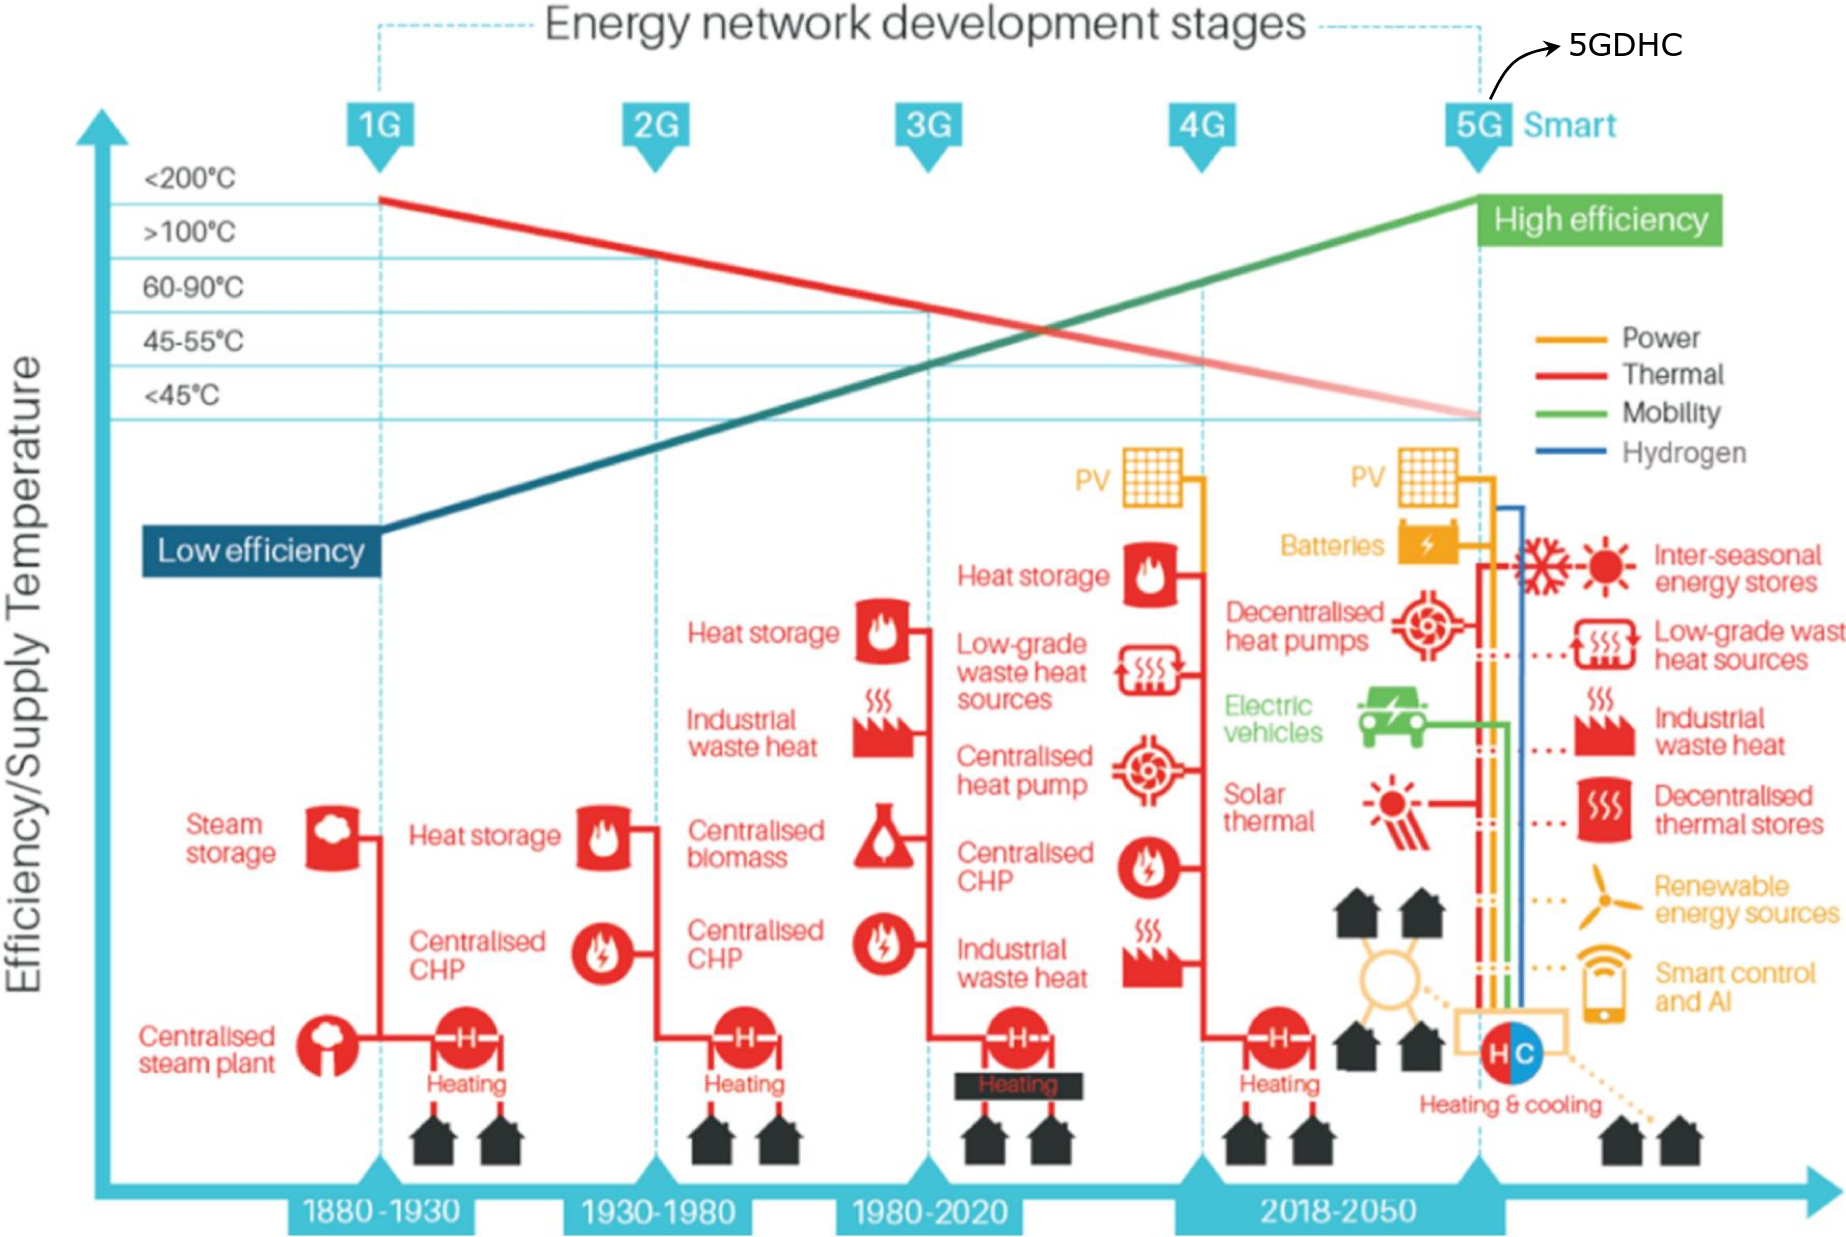
\includegraphics[\lw]{media/th-generations.png}

\subsubsection{Conventional network vs 5GDHC}
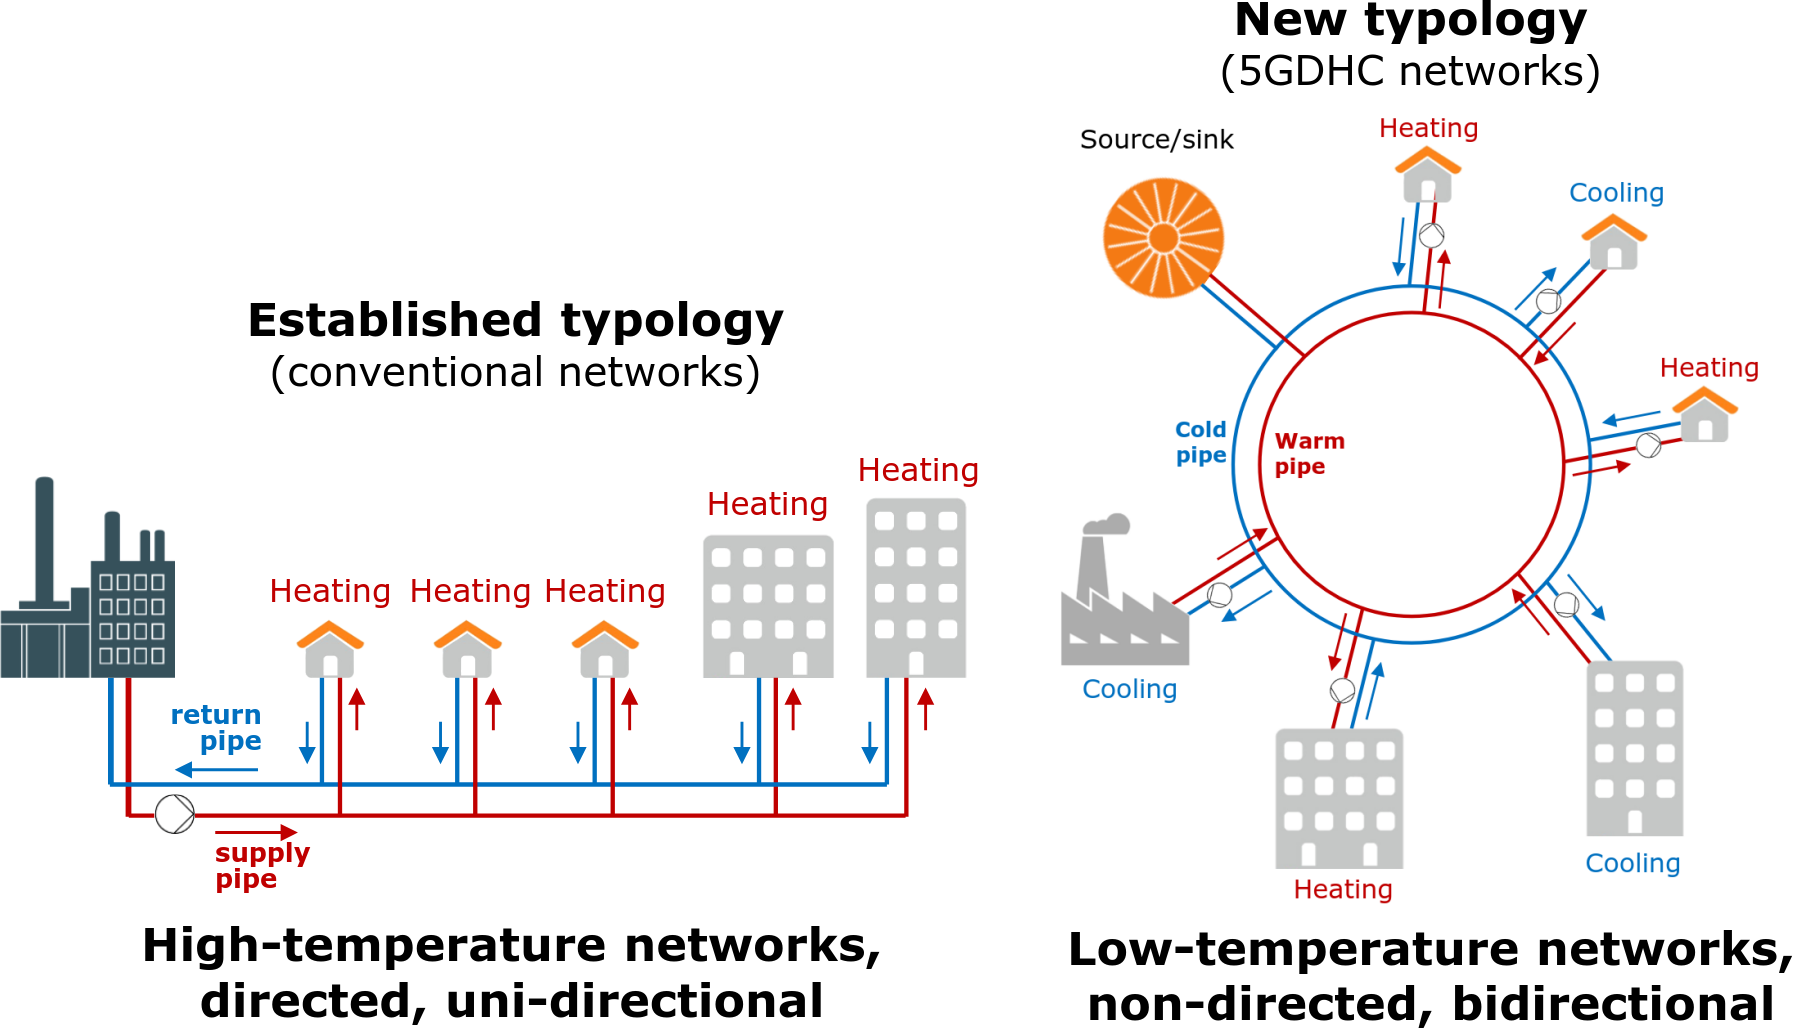
\includegraphics[\lw]{media/5gdhc.png}

\subsubsection{Pipe size}
\begin{center}
  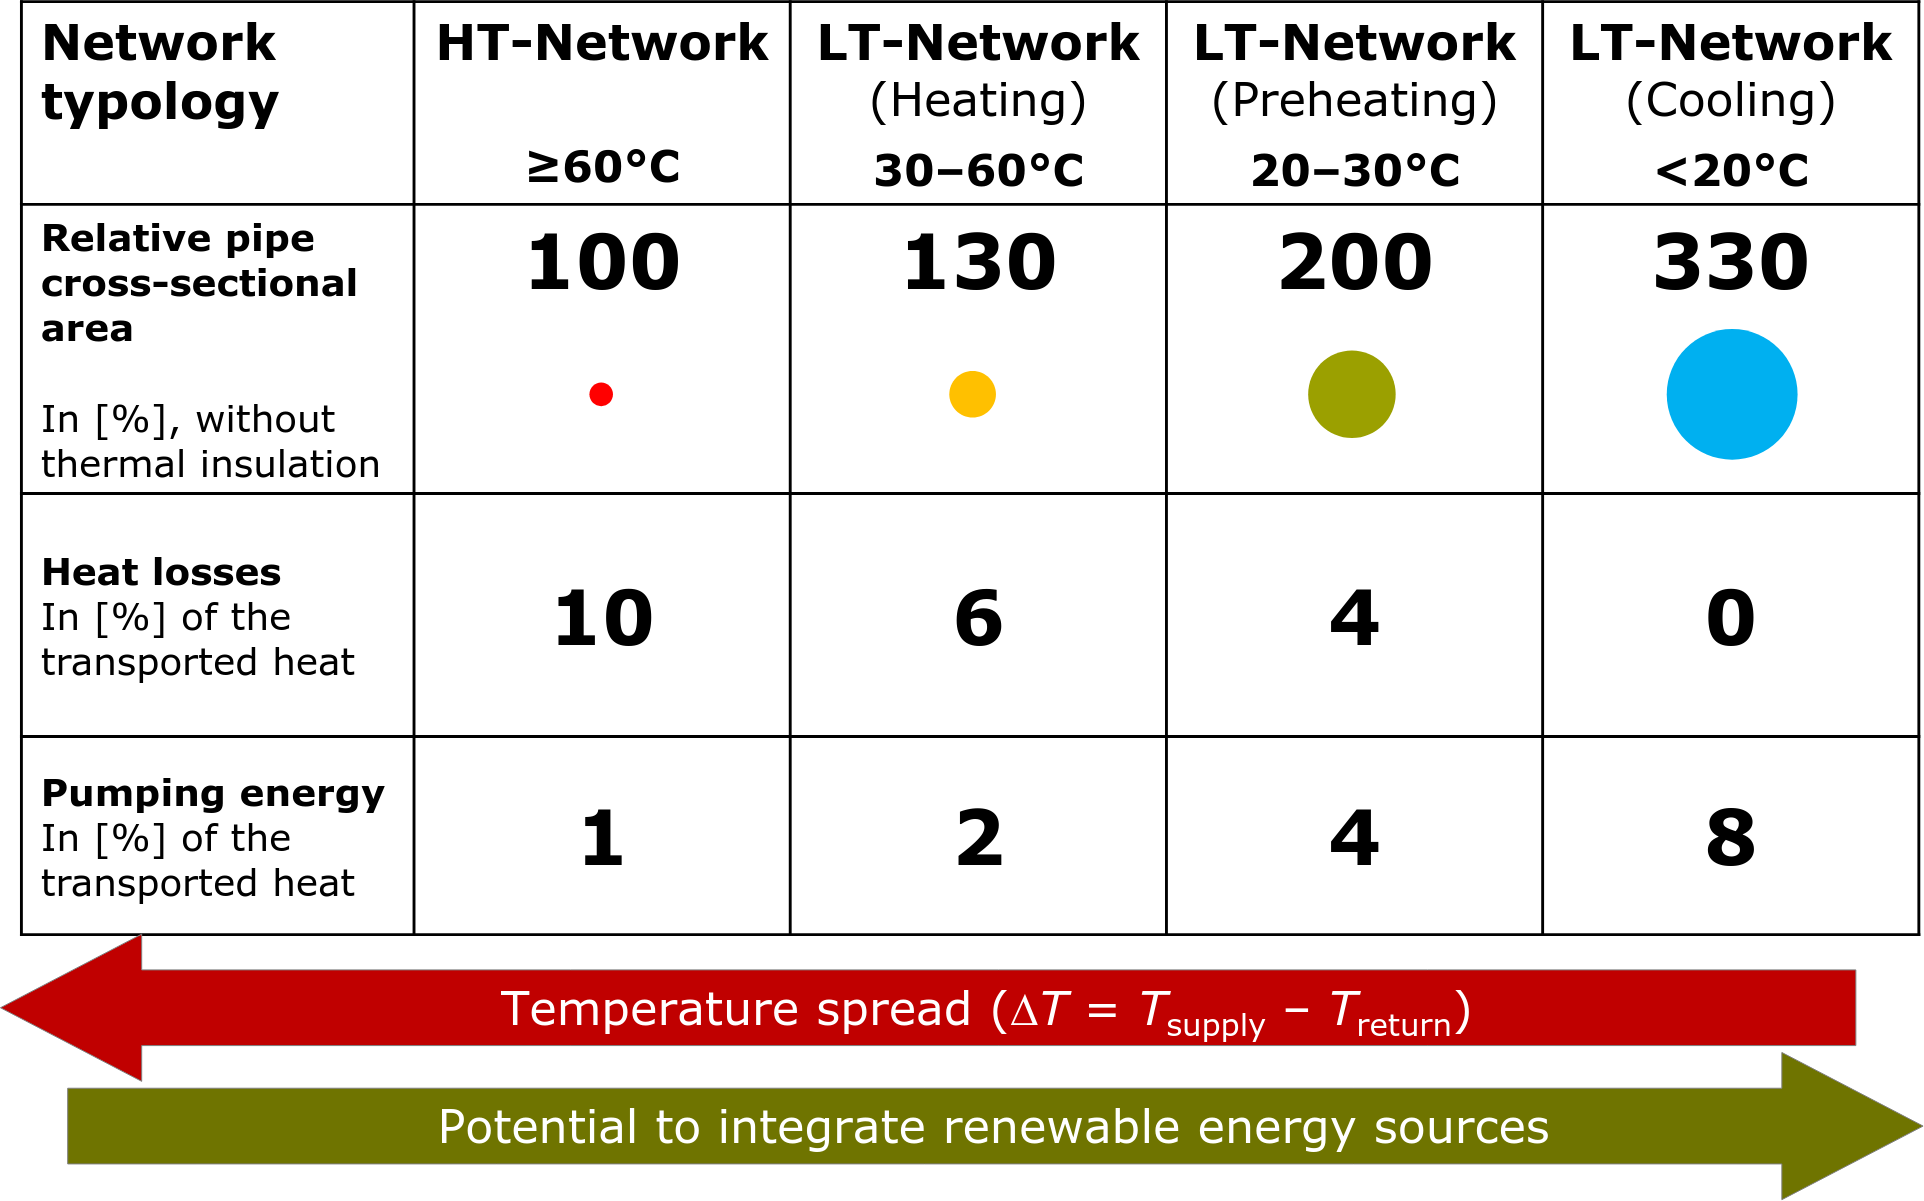
\includegraphics[\lw=.85]{media/pipe-size.png}
\end{center}

\subsection{Potential of district heating in CH}
\begin{itemize}
  \item CH: $\sim 1400$ thermal networks, $>9$ TWh/a heat; mostly HT
  \item Main sources today: waste incineration (W2E), biomass, gas, environmental/waste heat + HP
\end{itemize}

\subsubsection{Outlook 2050 (CH)}
\begin{itemize}
  \item Swiss building stock = 50\% of primary energy consumption
  \item More lakes, rivers, groundwater, geothermal, wastewater, environmental heat
  \item Increase of share of renewables, security of energy supply, and domestic value creation
  \item Decrease of CO$_2$ emissions
  \item DH potential: $\sim 17$ TWh/a; likely where heat density is high
\end{itemize}

\subsection{Climate and cooling}
\begin{itemize}
  \item Climate change: HDD decrease, CDD increase strongly
  \item Swiss service sector cooling demand forecast: 5--7 times today's demand by 2050. Cooling demand rises
  \item DHC with lakes/rivers/groundwater can provide efficient cooling and heat-source regeneration
\end{itemize}

\newcolumn
\section{Temperatures and pipes}
\subsection{Pipe types in district heating}
\begin{itemize}
  \item Plastic jacket pipes: steel process pipe, PUR insulation $\lambda\sim0.03$ W/(mK), PE jacket, up to 140\cel, single or dual pipes
  \item KMR/Premant: steel pipe, up to 140\cel
  \item Calpex: plastic pipe, up 90\cel
  \item Coolmant: plastic pipe, up to 40\cel
  \item 5GDHC: uninsulated plastic pipes at very low temperature
  \item Heat losses decrease with lower network temperature and better insulation
\end{itemize}

\subsection{District heating characteristics}
\subsubsection{Heat sources}
{\footnotesize
  \begin{tabularx}{\columnwidth}{@{}XX@{}}
  \toprule
  \textbf{Heat sources} & \textbf{Typical temperature / medium}\\
  \midrule
  Waste incineration heat & >120\cel\\
  \hline Wood firing & Hot water, supply >110\cel, steam\\
  \hline CHP unit & Supply <120\cel, typical 90\cel\\
  \hline \makecell[l]{Lake water, rivers, groundwater,\\shallow geothermal} & Supply <60\cel\\
  \hline Waste heat, sewage water & Supply <60\cel\\
  \bottomrule
\end{tabularx}}

\subsubsection{Choice of supply temperature}
{\footnotesize
  \begin{tabularx}{\columnwidth}{@{}lX@{}}
  \toprule
  \textbf{Criterion} & \textbf{Implication}\\
  \midrule
  Heat demand characteristics & \makecell[l]{Buildings old/new, industry,\\hospitals}\\
  \hline Heat source & Available temperature\\
  \hline Steam from steam turbine (CHP) & \makecell[l]{Supply temp. as low as possible\\for high electrical efficiency}\\
  \hline Size of network & Influence of heat losses\\
  \bottomrule
\end{tabularx}}

\subsubsection{Temperature spread}
\[\Delta T = T_\text{supply} - T_\text{return}\]
{\footnotesize
  \begin{tabularx}{\columnwidth}{@{}lX@{}}
  \toprule
  \textbf{Criterion} & \textbf{Effect}\\
  \midrule
  Large $\Delta T$ & \makecell[l]{Lower mass flow, smaller pipes,\\lower pumping energy}\\
  \hline Small $\Delta T$ & \makecell[l]{Higher COP for HP/chillers in 5GDHC,\\but higher mass flow}\\
  \hline Half $\Delta T$ & Double mass flow for same heat power\\
  \hline High supply temp. & Higher heat losses, but larger $\Delta T$ possible\\
  \hline Low supply temp. & \makecell[l]{65\cel: limit for conventional heating/DHW\\35\cel: low-T heating, eg. underfloor}\\
  \hline Low return temp. & \makecell[l]{Efficient CHP/cogeneration, larger $\Delta T$,\\low-T waste heat usable}\\
  \hline 5GDHC/anergy & \makecell[l]{Small $\Delta T$ helps high HP/chiller COP;\\large $\Delta T$ helps high thermal load}\\
  \bottomrule
\end{tabularx}}

\newcolumn
\section{Heat demand and economics}
\subsection{Economic feasibility of thermal networks}
\subsubsection{Linear heat density}
\[q_L = \frac{Q_\text{year}}{L}\ \left[\text{MWh}/(\text{km}\cdot\text{a})\right]\]
\begin{itemize}
  \item Linear heat density: annual heat demand per pipe length
  \item \textbf{Rough profitability criterion:} $q_L > 2000$ MWh/(km$\cdot$ a)
  \item Heat/power density: max. heating power per area; rough criterion $\sim 50$ MW/km$^2$
  \item Connection rate: share of units connected in an area
  \item Annual full-load hours: $h_\text{FL} = Q_\text{year}/P_\text{sub}$; typical residential $\sim 2000$ h
\end{itemize}

\subsubsection{Reduced linear heat density}
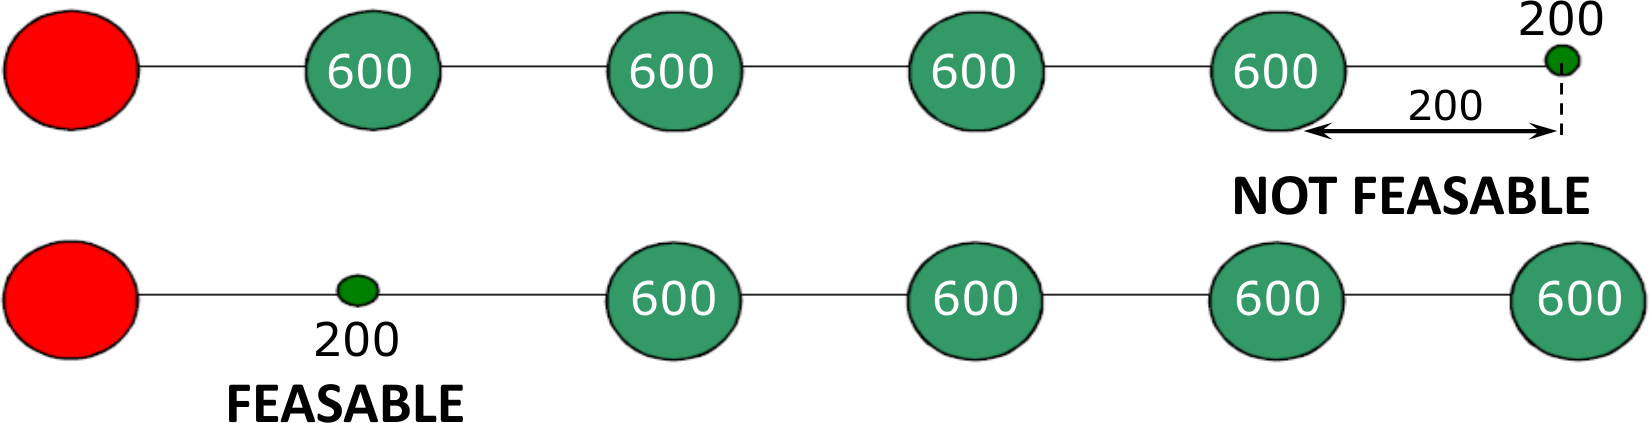
\includegraphics[\lw]{media/DHC-FEASABILITY.png}

\subsection{Load duration curve}
\begin{center}
  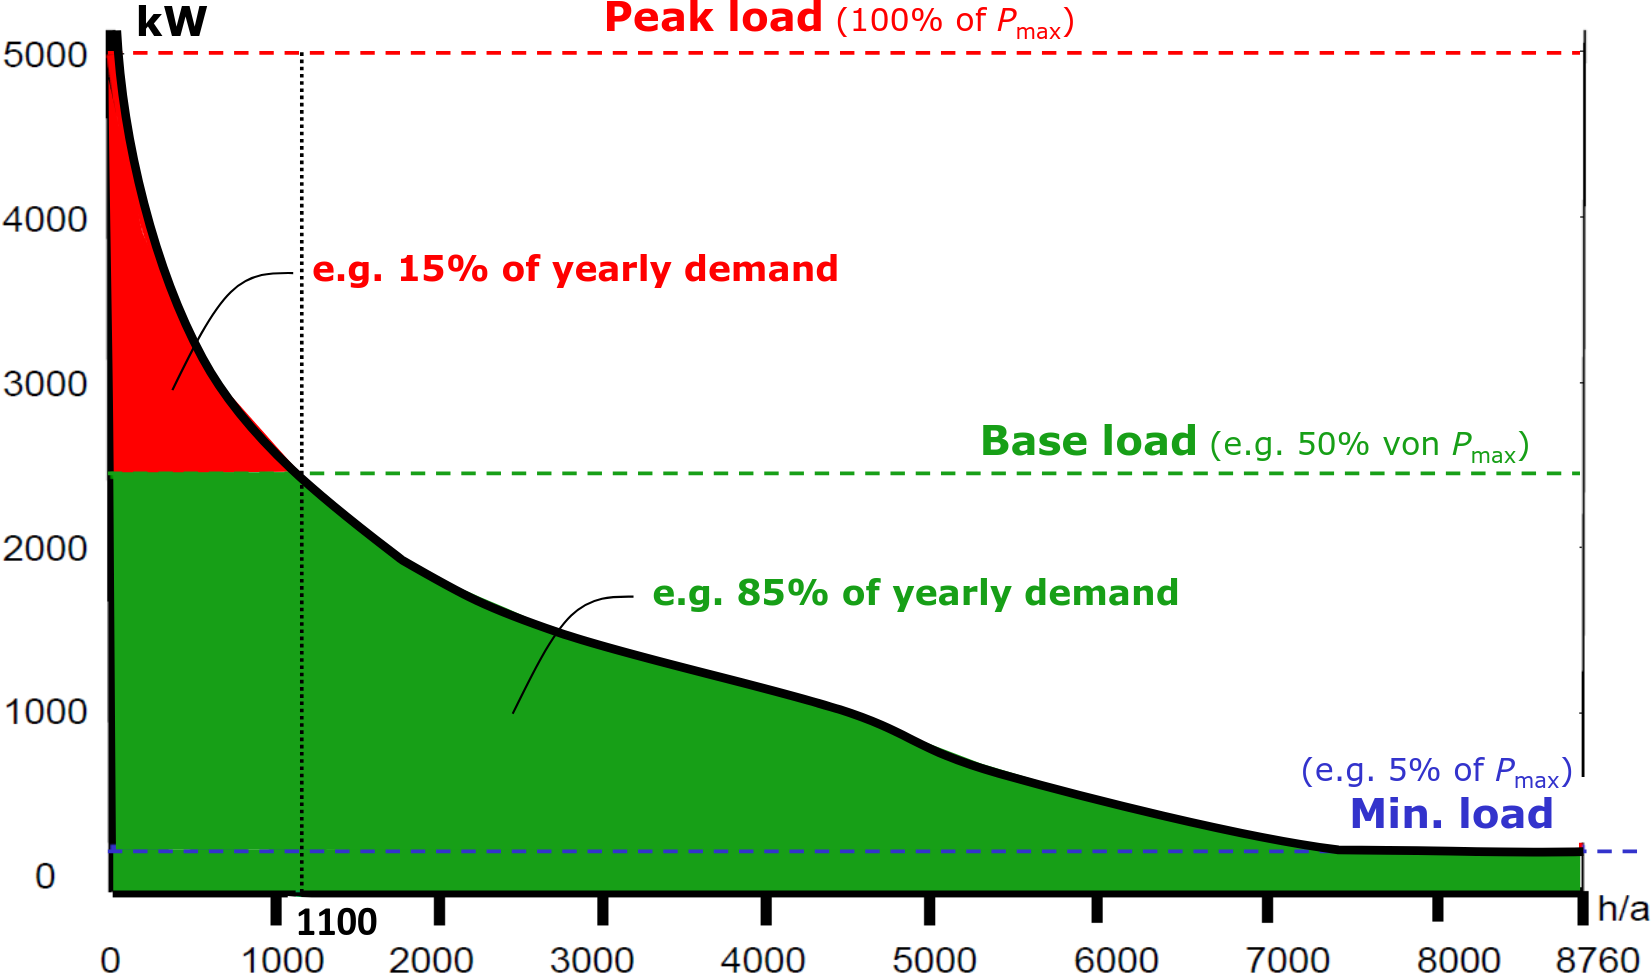
\includegraphics[\lw=.7]{media/load-type.png}
\end{center}
\vspace*{-.2cm}
\begin{itemize}
  \item Load sorted by frequency/duration over the year
  \item Area under curve = annual heat demand
  \item Base load covers many hours and much energy; peak load covers few hours
  \item Heat storage can shift short peak loads and reduce peak generator capacity
\end{itemize}

\section{Thermal power and sizing}
\subsection{Power and mass flow}
\begin{gather*}
  \dot Q = \dot m c_p (T_\text{supply} - T_\text{return})= \dot m c_p \Delta T\\
  \dot m = \frac{\dot Q}{c_p\Delta T}
\end{gather*}

\subsection{Required network (nominal) power}
\[\dot Q_\text{req} = \dot Q_\text{sub}\cdot f_\text{div} + \dot Q_l\]
\begin{itemize}
  \item $\dot Q_\text{sub}$: subscribed/connected customer power
  \item $\dot Q_l$: network heat losses
  \item In classic DH (90\cel): $\dot{Q}_l \approx 2\% \cdot \dot{Q}_\text{req}$
\end{itemize}

\subsection{Diversity factor (or simultaneity factor)}
\[f_\text{div} = \frac{\text{power drawn}}{\text{subscribed power}} = \frac{\sum_i \dot Q_i(t_\text{max})}{\sum_i \dot Q_{\text{sub},i}}\]
\begin{itemize}
  \item Consumers do not peak simultaneously; network power lower than sum of subscribed powers
  \item Diversity reduces required generation and pipe dimensions
\end{itemize}
\[f_\text{div} = a + \frac{b}{1+\left(\dfrac{n}{c}\right)^d}\]
where:\\
$a = 0.4497$, $b = 0.5512$, $c = 53.8438$, $d = 1.7627$, $n =$ customers

\subsection{Peak load and reserves}
\[
  P_P = P_\text{sub}\cdot f_\text{div} + P_L - P_S
\]
\begin{itemize}
  \item $P_P$: peak load coverage; $P_S$: base source power; $P_L$: losses
  \item Maintain supply if largest generator fails ($n-1$)
  \item Typical reserve agreement: 100\% network power for critical/larger grids; lower possible if accepted
\end{itemize}

\section{Hydraulics}
\subsection{Pressure loss}
\[\Delta p = \lambda\frac{L}{D}\frac{\rho v^2}{2}\quad ;\quad Re = \frac{\rho v d}{\mu} = \frac{vd}{\nu}\]
\begin{itemize}
  \item $\lambda=f(Re,k/D)$ depends on flow regime and pipe roughness
  \item For same pipe and similar flow regime: $\Delta p \propto v^2$
  \item Scaling: $\Delta p_2 = \Delta p_1\left(\dfrac{v_2}{v_1}\right)^2$
\end{itemize}
\subsubsection{Graphical visualization}
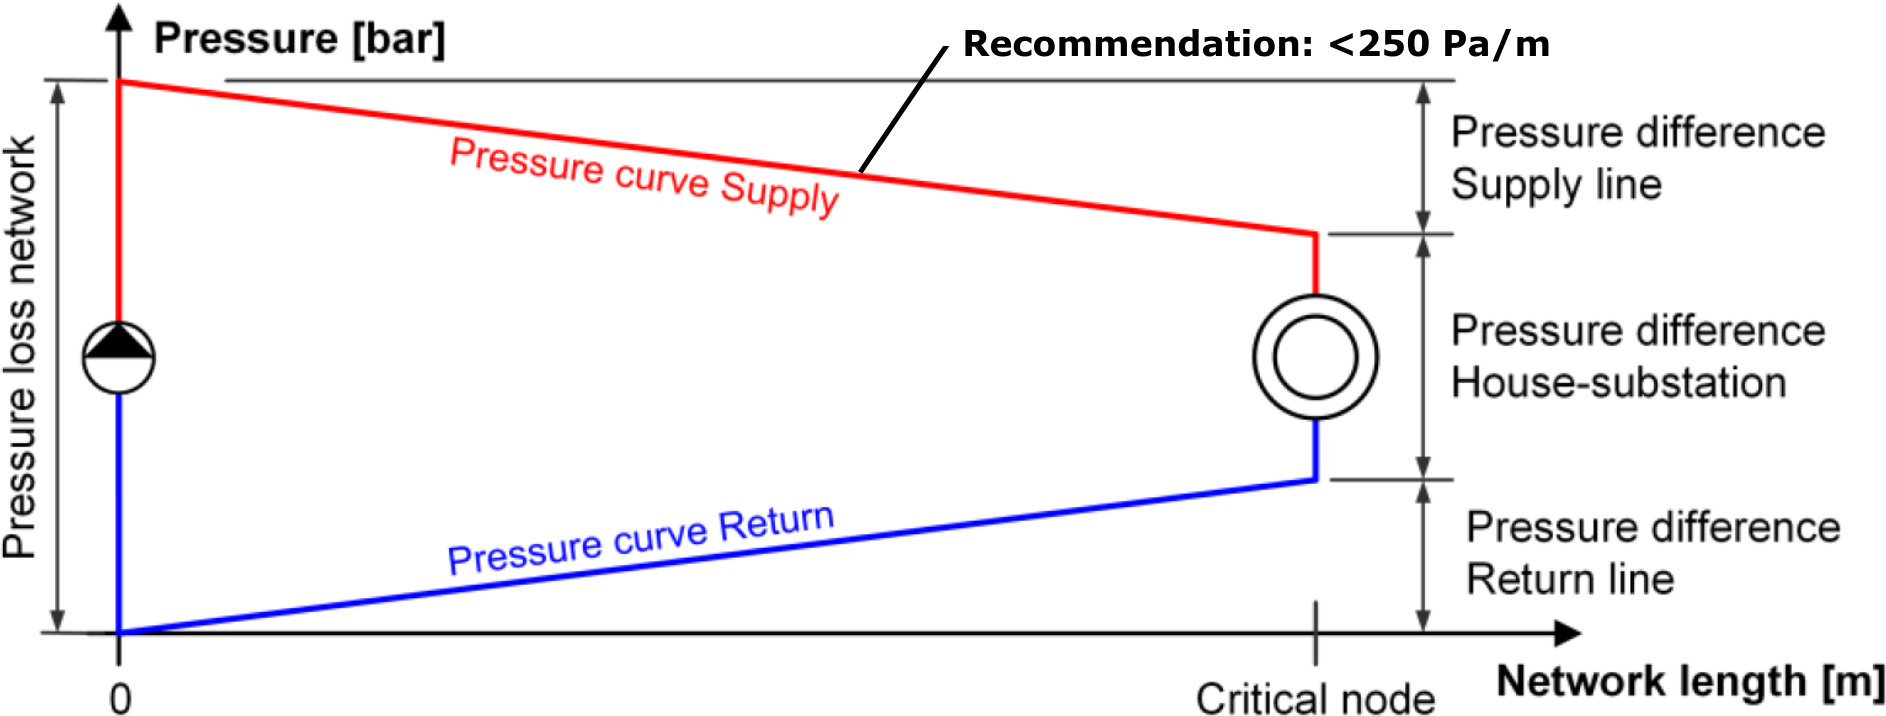
\includegraphics[\lw]{media/pressure-loss.png}

\subsection{Pumps and pressure}
\begin{itemize}
  \item Transfer stations need differential pressure, typically $\sim 0.7$--1 bar
  \item Network pressure must stay above vapor pressure plus safety margin at highest point
  \item Pump redundancy examples: $2\times100\%$, $3\times50\%$, $4\times33\%$
  \item Booster pumps can reduce maximum network pressure and central pump power
\end{itemize}

\newcolumn
\section{District heating exercise}
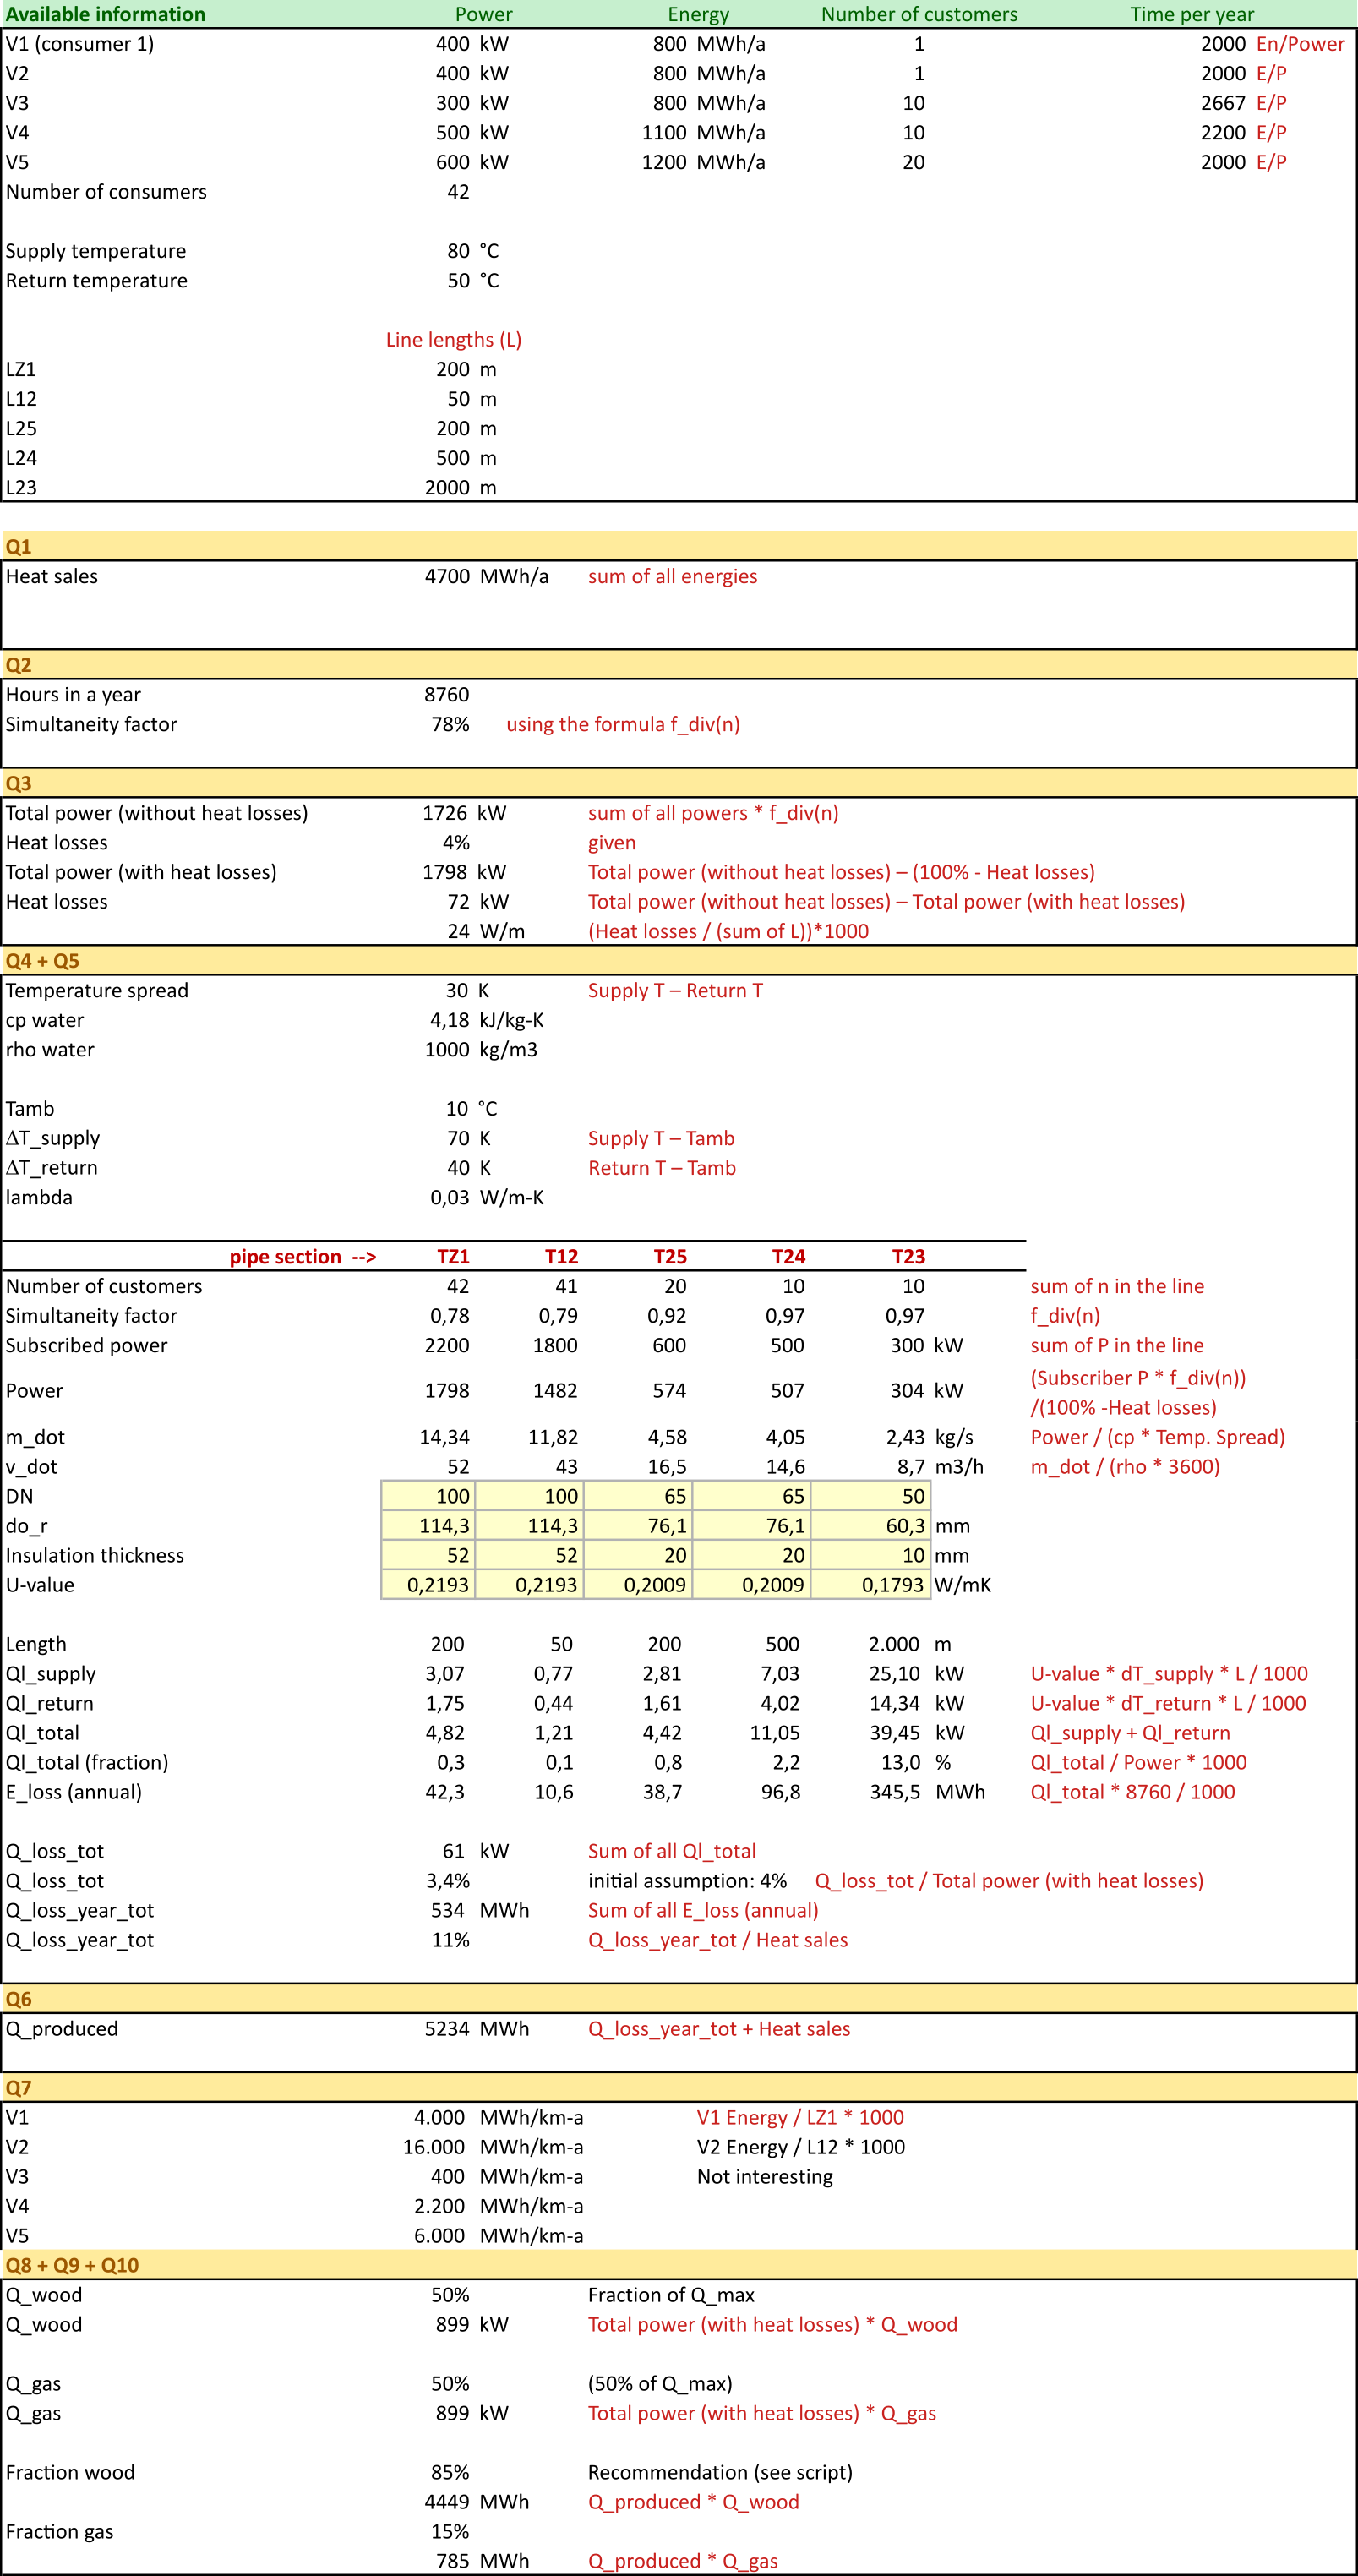
\includegraphics[\lw]{media/district-heating-exercise.png}

\section{Losses and cooling}
\subsection{Heat loss during operation}
\[q = U\cdot \left(T_B - T_E\right)\ \left[\text{W/m}\right]\]
where:
\vspace*{-.2cm}
\begin{itemize}
  \item $U =$ heat transfer coefficient [W/mK]
  \item $T_B =$ avg. T between VL/RL [\cel]
  \item $T_E =$ avg. ground temperature [\cel]
\end{itemize}

\subsection{Temperature drop along pipe}
\[\Delta T = \frac{\dot Q_l}{\dot m c_p}\qquad \text{or} \qquad\Delta T = \frac{q_l L}{\dot m c_p}\]
\begin{itemize}
  \item Low demand periods \to low $\dot m$ \to larger cooling of supply pipe
  \item Summer DHW-only operation can suffer larger temperature drop along the network
\end{itemize}

\subsection{Heat loss through insulation}
\[\dot Q = \frac{2\pi L\Delta T}{(1/\lambda)\ln(d_a/d_i)}\]
\begin{itemize}
  \item $d_a,d_i$: outer/inner insulation diameters; $L$: pipe length
  \item Losses scale with temperature difference and length; earth cover reduces losses somewhat
  \item Lower network temperatures reduce distribution losses
\end{itemize}

\subsection{Cooling of pipes}
\[T_i = T_u + \left(T_{io} - T_u\right)\exp\left(-\dfrac{1}{\dot{m} c_p R_{ges}}\right)\]
where:
\vspace*{-.2cm}
\begin{itemize}
  \item $T_i =$ Pipe T after a distance L
  \item $T_u =$ Ambient T
  \item $T_{io} =$ Pipe T at the source
  \item $R_{ges} =$ Thermal resistance [K/W]
\end{itemize}

\part{SW 14 + 15: Cost benefit analysis}

\section{CBA basics}
\begin{itemize}
  \item Cost-benefit analysis (CBA/BCA): accounting framework to compare project benefits and costs
  \item Societal CBA: aim is public welfare, not profit maximisation
  \item Project CBA: company/project perspective; include all relevant financial costs/benefits
  \item Can include market and non-market goods via shadow prices
\end{itemize}

\subsection{CBA workflow}
\begin{enumerate}[label=\arabic*.]
  \item Define scope, assumptions, perspective, period, actors
  \item Identify alternatives/baseline and quantify costs/benefits
  \item Select discount rate and calculate present values
  \item Compare alternatives using NPV or benefit-cost ratio
  \item Discuss uncertainties, risks, and sensitivity
\end{enumerate}

\section{1. Definition of scope and assumptions}
\begin{itemize}
  \item State problem and define perspective (societal vs project)
  \item Proportionate analysis: depth of CBA $\propto$ expected effect size
  \item Find C/B stakeholders: municipality, company, users, society
\end{itemize}

\subsection{Partial equilibrium analysis}
\begin{itemize}
  \item Analyse one market separately from the rest of the economy
  \item Valid when effects on other markets are negligible
  \item e.g. town compares buying a garbage truck vs. outsourcing collection
\end{itemize}

\subsection{General equilibrium analysis}
\begin{itemize}
  \item Analyse all affected markets at the same time
  \item Includes effects on transport, plastics, labour, and other linked markets
  \item e.g. national waste strategy or nationwide oil tax
\end{itemize}

\section{2. Alternatives / Quantification of C/B}
\begin{itemize}
  \item Identification of alternatives or baseline
  \item Translation of costs and benefits in monetary units
  \item Goods/services traded in the market vs. non-market costs and benefits
\end{itemize}

\subsection{Shadow prices and externalities}
\subsubsection{Shadow price}
Assigned value for a non-market good, e.g. users' time savings.
Also used when market prices do not reflect true social value.
If the shadow price exceeds the market price, hidden costs indicate a negative externality.

\subsubsection{Negative externality}
Third-party cost not included in transaction, e.g. noise or pollution
\begin{center}
  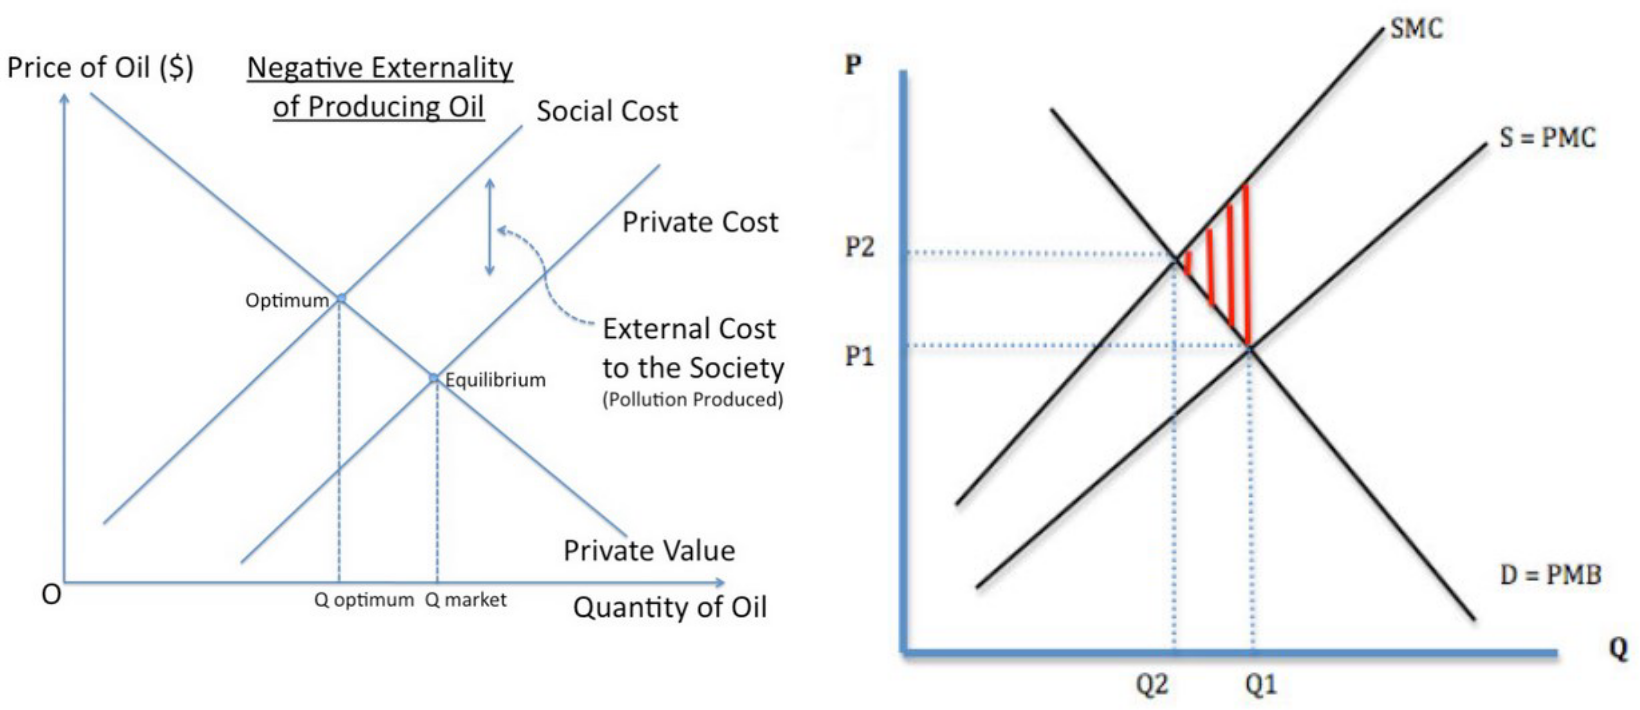
\includegraphics[\lw]{media/negative-externality.png}
\end{center}

\subsubsection{Positive externality}
A third party gains an additional benefit without being part of the transaction.
The social value is higher than the private transaction value, e.g. technology spillovers
where society benefits from new knowledge beyond the company itself.

\subsubsection{Market failure}
Market price does not reflect full social cost/benefit

\subsection{WTP and WTA}
\begin{itemize}
  \item Willingness-to-pay (WTP): amount someone pays to gain benefit or reduce harm
  \item Willingness-to-accept (WTA): compensation needed to accept a harm/loss
  \item WTA often higher than WTP; legal rights affect which measure is appropriate
  \item WTP is income constrained; WTA less directly constrained
\end{itemize}

\newcolumn
\subsection{Methods for determining WTP and WTA}
\subsubsection{Travel cost method}
\begin{itemize}
  \item Estimates WTP for recreational sites or environmental quality changes
  \item Travel time, travel expenses, and entry fees act as the implicit access price
  \item Higher travel cost usually means fewer visits; visit frequency reveals demand/WTP
  \item eg. national park with \$2.50 entry fee; individual WTP = entry fee + travel cost
  \item Average visitor demand gives the shadow price of one visit
  \item Shadow price $\times$ annual visitors = annual recreational value of the site
\end{itemize}

\subsubsection{Contingent method}
\begin{itemize}
  \item Stated-preference method: survey directly asks WTP/WTA for an environmental service
  \item "Contingent" because valuation depends on a hypothetical scenario
  \item Useful for monetising non-market goods when no market behaviour is observable
  \item Case: reservoir outflow decision trades hydropower generation against recreational water quality
  \item Survey estimates visitors' WTP for better water quality
  \item Optimum outflow: compare water-quality value with lost hydropower value
\end{itemize}

\subsubsection{Conjoint analysis}
\begin{itemize}
  \item Similar to contingent valuation, but compares bundles of attributes instead of one good
  \item Example options combine water quality, electricity mix, and lake outflow impacts
  \item Respondents choose their preferred bundle
  \item Regression analysis estimates the value of each individual attribute
\end{itemize}

\subsubsection{Challenges with WTP/WTA methods}
\begin{itemize}
  \item Sample bias: surveyed group may not represent the average population
  \item Response bias: people may overstate or understate their true WTP/WTA
  \item Legal rights determine whether WTP or WTA is appropriate
  \item Airport-noise example: WTP asks what residents pay for noise reduction; WTA asks compensation to accept noise
  \item WTP is income constrained, WTA is less constrained and often gives higher shadow prices
\end{itemize}

\section{3. Discount rate and present value}
\begin{itemize}
  \item Costs/benefits occur at different times: initial investment, future gains, future O\&M
  \item Cash flows are spread over time, not paid as one lump sum
  \item Time value of money: money today is worth more because it can earn interest
  \item Therefore, yearly cash flows must be discounted to present value
\end{itemize}

\subsection{Present value}
\[PV_t = \dm \sum_{t=0}^N\frac{F_t}{(1+r)^t}\]
\begin{itemize}
  \item $F_t$: cash flow at time $t$; $r$: discount rate; $t$: year
  \item Future cash flows are worth less than immediate cash flows
  \item High discount rates penalise projects with near-term costs and future benefits
  \item Recommended rates vary widely, often 2--10\%; use sensitivity analysis
\end{itemize}

\subsection{Real vs. nominal}
\[r_\text{real} \approx r_\text{nominal} - \pi\]
\begin{itemize}
  \item Use comparable monetary units: nominal or constant prices
  \item For constant prices, subtract expected inflation $\pi$ from nominal rate
  \item Example: nominal 8\%, inflation 5\% $\to$ real rate $\approx 3\%$
\end{itemize}

\section{4. Comparing alternatives}
\subsection{Net present value (NPV)}
\[NPV = \sum_{t=0}^{N}\frac{B_t-C_t}{(1+r)^t}= PV(B)-PV(C)\]
\begin{itemize}
  \item NPV = present value of benefits - present value of costs
  \item $NPV>0$: project passes CBA test
  \item $NPV<0$: reject from the chosen perspective
  \item Good absolute measure when alternatives differ in size
\end{itemize}

\subsection{Benefit-cost ratio (B/C)}
\[B/C = \frac{PV(B)}{PV(C)}\]
\begin{itemize}
  \item $B/C>1$: financially acceptable
  \item Drawback: can favour small projects with high ratio but low absolute benefit
  \item Use together with NPV when project scales differ
  \item e.g. Project A may cost \$100'000 and have lower $B/C$ than project B costing \$100, but A can still create more total net benefit
\end{itemize}

\section{5. Uncertainty and risk}
\begin{itemize}
  \item Sensitivity analysis: vary uncertain parameters and observe output
  \item Important parameters: discount rate, fuel price, demand, lifetime, investment cost
  \item CBA result depends strongly on scope, valuation, and assumptions
\end{itemize}

\newcolumn
\section{Example: garbage truck}
\subsection{Setup}
\begin{itemize}
  \item Lucerne compares buying a garbage truck vs. outsourced collection
  \item Perspective: city treasury; no resident externalities included
  \item Period: 5 years; real discount rate: 3\%; partial equilibrium
\end{itemize}

{\footnotesize
\begin{tabularx}{\columnwidth}{@{}lX@{}}
  \toprule
  \textbf{Item} & \textbf{Value}\\
  \midrule
  Truck purchase & 60'000 EUR initial cost\\
  Driver + maintenance + fuel & 38'000 EUR/a\\
  Scrap value & 12'000 EUR in year 5\\
  Year 5 truck cost & 26'000 EUR\\
  Contract cost & 50'000 EUR/a\\
  Undiscounted difference & 12'000 EUR saved over 5 years\\
  \bottomrule
\end{tabularx}}

\subsection{Results}
{\footnotesize
\begin{tabularx}{\columnwidth}{@{}lX@{}}
  \toprule
  \textbf{Case} & \textbf{Result}\\
  \midrule
  3\% discount rate & $NPV=5'308$ EUR $\to$ buy truck\\
  $B/C$ at 3\% & $228'985/223'678 = 1.024 > 1$\\
  7\% discount rate & $NPV=-2'242$ EUR $\to$ do not buy\\
  Fuel cost 3'000 EUR/a & $NPV=-3'852$ EUR at 3\%\\
  \bottomrule
\end{tabularx}}

\begin{itemize}
  \item Same undiscounted savings can become unattractive after discounting
  \item Fuel-cost and discount-rate assumptions change the decision
  \item CBA supports decisions but does not remove uncertainty
\end{itemize}

\part{SW 2 -- 5: exercises}

\section{SW2: Renewable Energy Sources 1}
\begin{exercisebox}[Exercise: Solar area for world energy demand]
  World energy demand: $183'230$ TWh/a. Average solar irradiance: $1361$ W/m$^2$.
  PV efficiency: $\eta=25\%$. Earth area: $510'100'000$ km$^2$, land share: 29\%.
  \begin{enumerate}[label=\alph*.]
    \item How much PV area is required to cover the world energy demand?
    \item What share of world land surface is this?
  \end{enumerate}
  \hr
  \begin{enumerate}[label=\alph*.]
    \item $A=\frac{183'230\cdot10^{12}\text{ Wh}}{1361\text{ W/m}^2\cdot8760\text{ h}\cdot0.25}
      \approx 6.15\cdot10^{11}\text{ m}^2 = 615'000\text{ km}^2$
    \item $A_\text{land}=510'100'000\text{ km}^2\cdot0.29\approx147.9\cdot10^6\text{ km}^2$\\
      $\frac{615'000}{147.9\cdot10^6}\cdot100\approx0.42\%$
  \end{enumerate}
\end{exercisebox}

\begin{exercisebox}[Exercise: Sun radiation]
  Given $\sigma=5.670\cdot10^{-8}$ W/(m$^2$K$^4$), $T_\text{sun}\approx5780$ K.
  \begin{enumerate}[label=\alph*.]
    \item Calculate the specific radiation power at the sun surface.
    \item Calculate total radiation power of the sun.
    \item Estimate solar irradiance at Earth distance.
    \item Estimate average radiation power over Earth surface.
  \end{enumerate}
  \hr
  \begin{enumerate}[label=\alph*.]
    \item $E_\text{sun}=\sigma T^4\approx6.33\cdot10^7$ W/m$^2$
    \item $P_\text{sun}=E_\text{sun}\cdot4\pi R_\text{sun}^2\approx3.85\cdot10^{26}$ W
    \item Inverse-square scaling gives $E_\text{solar}\approx1354$ W/m$^2$
    \item Average over sphere: $\bar E_\text{Earth}\approx E_\text{solar}/4\approx340$ W/m$^2$
  \end{enumerate}
\end{exercisebox}

\section{SW3: Renewable Energy Sources 2}
\begin{exercisebox}[Exercise: Run-of-river plant Lucerne]
  Given: head $h=2$ m, two Kaplan turbines with $Q=29$ m$^3$/s each,
  river speed $v=2$ m/s, actual yearly production $2400$ MWh/a, $\eta_\text{el}=0.9$.
  \begin{enumerate}[label=\alph*.]
    \item Compute hydraulic power and kinetic river-power share.
    \item Compute yearly electricity at full load.
    \item Compare with actual production and explain the gap.
  \end{enumerate}
  \hr
  \begin{enumerate}[label=\alph*.]
    \item $Q_\text{tot}=58$ m$^3$/s\\
      $P_h=\rho gQh=1000\cdot9.81\cdot58\cdot2\approx1.14$ MW\\
      $P_k=\frac12\rho Qv^2=\frac12\cdot1000\cdot58\cdot2^2\approx0.116$ MW
    \item $E_\text{full}=P_h\eta\cdot8760\text{ h}\approx1.14\cdot0.9\cdot8760\approx8970$ MWh/a
    \item Actual output is lower due to variable/low head and flow, downtime, ecological constraints, and non-full-load operation.
  \end{enumerate}
\end{exercisebox}

\begin{exercisebox}[Exercise: Storage power plant Goeschenen]
  Given: storage lake volume $V=75\cdot10^6$ m$^3$, Pelton turbines $3\cdot41=123$ MW,
  $\eta=0.9$, household demand $4500$ kWh/a. Head $h$ is not given on the extracted slide.
  \begin{enumerate}[label=\alph*.]
    \item Calculate potential energy and produced electricity.
    \item Estimate number of households supplied.
    \item Estimate minimum depletion time.
  \end{enumerate}
  \hr
  \begin{enumerate}[label=\alph*.]
    \item $E=\rho gVh$, \quad $E_\text{el}=\eta\rho gVh$; insert known/given head $h$ if available.
    \item $N_\text{HH}=\frac{E_\text{el}[\text{kWh}]}{4500\text{ kWh/a}}$
    \item $t_\text{min}=\frac{E_\text{el}}{123\text{ MW}}$
  \end{enumerate}
\end{exercisebox}

\section{SW4: Energy Storage}
\begin{exercisebox}[Exercise: Capacitor]
  Given: $U=10$ V, $r=20$ cm, $d=5$ mm, $P_\text{LED}=75$ mW, glass $\varepsilon_r=4.7$.
  \begin{enumerate}[label=\alph*.]
    \item Energy stored with air between plates?
    \item How long can an LED burn with this energy?
    \item Energy stored with glass dielectric?
  \end{enumerate}
  \hr
  \[
    C=\varepsilon\frac{A}{d}, \qquad E=\frac12CU^2, \qquad t=\frac{E}{P}
  \]
  \begin{enumerate}[label=\alph*.]
    \item Air: $E\approx1.1\cdot10^{-8}$ J
    \item $t=1.1\cdot10^{-8}/0.075\approx1.5\cdot10^{-7}$ s
    \item Glass: $E\approx5.2\cdot10^{-8}$ J
  \end{enumerate}
\end{exercisebox}

\begin{exercisebox}[Exercise: Stratified sensible tank]
  Compare energy and exergy for tanks with 2 m thermocline, 10 m thermocline, and fully mixed state.
  Also discuss replacing water by gravel. Given: $r=8$ m, $H=40$ m,
  hot 90\cel, cold 30\cel, mixed 60\cel, ambient 18\cel, $c_p=4.18$ kJ/(kgK).
  \hr
  \begin{enumerate}
    \item Tank mass: \[m = \rho V = \rho\pi R^2 H\]
    \item Energy: \[Q = m\ c_p\left(T_\text{mix} - T_\text{amb}\right)\]
    \item Exergy:
    \begin{gather*}
      f(T) = \left(T-T_\text{amb} - t_\text{amb}\ln\frac{T}{T_\text{amb}}\right)\\[1ex]
      Ex = \frac{m\cdot c_p}{H}\left[h_cf(T_c) + h_hf(T_h) + \frac{h_\text{th}}{T_h - T_c} \integral[T_c][T_h][f(T)][T]\right]\\[1ex]
      \integral[T_c][T_h][f(T)][T] = \left[\frac{T^2}{2} - T_\text{amb}\cdot T\ln\frac{T}{T_\text{amb}}\right]_{T_c}^{T_h}
    \end{gather*}
  \end{enumerate}
  

\end{exercisebox}

\begin{exercisebox}[Exercise: Flywheel]
  Solid cylindrical flywheel: $m=50$ kg, $r=0.5$ m, $6000$ RPM. Load: 2 kW.
  \begin{enumerate}[label=\alph*.]
    \item Calculate moment of inertia.
    \item Calculate stored rotational kinetic energy.
    \item Calculate runtime at 2 kW.
  \end{enumerate}
  \hr
  \begin{enumerate}[label=\alph*.]
    \item $J=\frac12mr^2=\frac12\cdot50\cdot0.5^2=6.25$ kg m$^2$
    \item $\omega=2\pi\cdot6000/60\approx628$ rad/s\\
      $E=\frac12J\omega^2\approx0.5\cdot6.25\cdot628^2\approx1.23$ MJ
    \item $t=E/P=1.23\text{ MJ}/2\text{ kW}\approx615$ s $\approx10.3$ min
  \end{enumerate}
\end{exercisebox}

\section{SW5: Residential Buildings}
\begin{exercisebox}[Exercise: Residential energy bill]
  Estimate yearly household energy costs for heating, TV, phone charging, and showering.
  Use $C_\text{el}=P\cdot t\cdot c_\text{el}$ and $E=mc_p\Delta T$.
  Typical orders: heating 7000 kWh/a, hot water 3000 kWh/a, electricity 4000--5000 kWh/a.
  \hr
  Examples from slides:
  \begin{itemize}
    \item TV: 2 h/week, 32 kWh/1000 h $\to E\approx3.33$ kWh/a $\to$ about 1 CHF/a
    \item Phone: 10.28 Wh/day $\to E\approx3.75$ kWh/a $\to$ about 1.13 CHF/a at 0.30 CHF/kWh
    \item Shower: 8 min, 9 l/min, 365 showers/a, $\Delta T=30$ K\\
      $E\approx898$ kWh/a $\to$ about 269 CHF/a electricity plus water cost
  \end{itemize}
\end{exercisebox}

\begin{exercisebox}[Exercise: Heat pump ROI]
  Oil heating cost: 3500 CHF/a. Water-water heat pump investment: 27000 CHF.
  Thermal demand: 20000 kWh/a, COP $=3.5$, electricity price: 0.29 CHF/kWh.
  \begin{enumerate}[label=\alph*.]
    \item Calculate payback time and ROI.
    \item Would you recommend the heat pump?
  \end{enumerate}
  \hr
  \begin{enumerate}[label=\alph*.]
    \item $E_\text{el}=20000/3.5=5714$ kWh/a\\
      $C_\text{HP,el}=5714\cdot0.29\approx1657$ CHF/a\\
      Savings $=3500-1657=1843$ CHF/a\\
      $ROI=\frac{1843}{27000}=0.068=6.8\%$\\
      Payback $=\frac{27000}{1843}\approx14.6$ a
    \item Marginal: payback is close to heat-pump lifetime. Arguments: future heat-demand reduction,
      possible oil-price increase, PV can lower electricity cost.
  \end{enumerate}
\end{exercisebox}

\part{Renergia}
\begin{itemize}
  \item Waste has a high calorific value: roughly comparable with coal for the same mass
  \item Waste crane/loading cycles: about 3500 smartphone charges; truck unloading takes about 16 min
  \item Highest waste input after Christmas; observed maximum about 1700 t/day
  \item Typical plant output: about 50 MW
  \item Bottom ash/slag: about 20\% of input; about 10\% of slag is metal, including non-ferrous metals
  \item Metals are recovered from slag, e.g. at Uri/Attinghausen treatment facilities
  \item Combustion residues are water-cooled, limiting dust/wind dispersion and cooling material from about 110\cel
  \item Tubular heat exchangers last roughly 10 years; ash deposits require periodic cleaning to avoid blockage
  \item Flue gas cleaning: baking soda neutralises acidic gases; cloth/bag filters remove particles
  \item NO$_x$ reduction uses catalyst with AdBlue/ammonia; activated carbon removes remaining pollutants
\end{itemize}






































\end{multicols*}
\end{document}
